\documentclass{beamer}
\setbeamerfont{headline}{size=\footnotesize}

\mode<presentation>{
\usetheme{Montpellier}
\setbeamercovered{transparent}
\usecolortheme{lsc}
}

\mode<handout>{
  % tema simples para ser impresso
  \usepackage[bar]{beamerthemetree}
   % Colocando um fundo cinza quando for gerar transparências para serem impressas
  % mais de uma transparência por página
  \beamertemplatesolidbackgroundcolor{black!5}
}

\usepackage{fancyvrb}
\usepackage{pdfpages} % Pacote para incluir PDFs
\usepackage{amsmath, amssymb} % Para símbolos matemáticos
\usepackage{tikz} % Para diagramas
\usepackage{pgfplots} % Para gráficos
\usepackage{amsmath,amssymb}
\usepackage[brazil]{varioref}
\usepackage[english,brazil]{babel}
\usepackage[utf8]{inputenc}
\usepackage{fontawesome}
\usepackage{ccicons}

\usepackage{makecell} % Adicione isso no preâmbulo do documento

%\usepackage[latin1]{inputenc}
\usepackage{graphicx}
\usepackage{listings}
\usepackage{url}
\usepackage{colortbl}
\usepackage{caption}
\usepackage{tikz}
\usepackage{transparent}
\usepackage{multirow}
\usepackage{graphicx}
\usepackage{listings}
\usepackage{exercise,chngcntr}

\usepackage{listings}
\usepackage{xcolor}
\usepackage{tikz}
\usetikzlibrary{shapes, arrows.meta, positioning}


% Definição de cores para o código Python
\definecolor{codegreen}{rgb}{0,0.6,0}
\definecolor{codegray}{rgb}{0.5,0.5,0.5}
\definecolor{codepurple}{rgb}{0.58,0,0.82}
\definecolor{backcolour}{rgb}{0.95,0.95,0.92}
% Configuração do estilo do código Python
\lstdefinestyle{mystyle}{
    xleftmargin=0pt,           % Aumenta a margem esquerda
    xrightmargin=10pt,          % Aumenta a margem direita
    frame=single,               % Adiciona um quadro ao redor do código
    framesep=10pt,              % Espaço entre o quadro e o código
    % Outras configurações do lstlisting...
    backgroundcolor=\color{backcolour},
    commentstyle=\color{codegreen},
    keywordstyle=\color{magenta},
    numberstyle=\tiny\color{codegray},
    stringstyle=\color{codepurple},
    basicstyle=\footnotesize\ttfamily,
    breakatwhitespace=false,
    breaklines=true,
    captionpos=b,
    keepspaces=true,
    %numbers=left,
    numbersep=5pt,
    showspaces=false,
    showstringspaces=false,
    showtabs=false,
    tabsize=2,
    basicstyle=\ttfamily, % Usa uma fonte de largura fixa para o código
    upquote=true,         % Tenta usar aspas retas se a fonte suportar,
    breakatwhitespace=false, % Quebra linhas em espaços em branco quando possível
}

\lstset{style=mystyle}


\beamertemplatetransparentcovereddynamic
\addtobeamertemplate{title page}{\centering{ 
\includegraphics[width=1.25cm]{figs/logo.png}}}{}
\title[]{Machine Learning}
\author[Elton Sarmanho]{ 
Professor: Elton Sarmanho\inst{1} 
\newline
E-mail: \href{mailto:eltonss@ufpa.br}{eltonss@ufpa.br}\newline
\href{https://github.com/eltonsarmanho}{\faGithub} \href{https://www.linkedin.com/in/elton-sarmanho-836553185/}{\faLinkedinSquare}\\
\ccbyncsa
}   
  \institute[UFPA]{
   \inst{1}%
     Faculdade de Sistemas de Informação - UFPA/CUNTINS
     }     
 
% Se comentar a linha abaixo, irá aparecer a data quando foi compilada a apresentação  
\date{\today}
\pgfdeclareimage[height= 1.25 cm]{inf}{figs/logo.png}
% pode-se colocar o LOGO assim
\logo{{\transparent{0.35}\pgfuseimage{inf}}}

% \AtBeginSection[]{
%   \begin{frame}<beamer>
%     \frametitle{Roteiro}
%     \tableofcontents[currentsection,currentsubsection]
%   \end{frame}  
% }

\setbeamertemplate{navigation symbols}{\insertframenavigationsymbol \insertsectionnavigationsymbol \insertbackfindforwardnavigationsymbol} 


\expandafter\def\expandafter\insertshorttitle\expandafter{%
  \insertshorttitle\hfill%
  \insertframenumber\,/\,\inserttotalframenumber}
  \renewcounter{Exercise}[section]
  \newcounter{Example}



\begin{document}

\setbeamertemplate{logo}{}
\begin{frame}
\titlepage
\end{frame}
%Começar mostrar Logo apos slide de titulo
\logo{{\transparent{0.35}\pgfuseimage{inf}}}

\begin{frame}
\frametitle{Roteiro}
\tableofcontents[sections={1-3}]
\end{frame}
\begin{frame}
\frametitle{Roteiro}
\tableofcontents[sections={4-6}]
\end{frame}

\begin{frame}
\frametitle{Roteiro}
\tableofcontents[sections={7-8}]
\end{frame}

\begin{frame}
\frametitle{Roteiro}
\tableofcontents[sections={9-10}]
\end{frame}
\begin{frame}{Licença}
    Este trabalho está licenciado sob a licença Creative Commons:

    \bigskip
    \ccbyncsa
\end{frame}
%Declaração das Imagens da Apresentação

%%%%%%%%%%%%%%%%%%%%%%%%%%%%%%%%%%%%%%%%
\section{Planejamento}

\begin{frame}
Nesta aula:

\begin{itemize}
 \item Vamos explorar os conceitos fundamentais de aprendizagem de máquina.
 \item Ter panorama sobre conceito.
 \item Códigos do livro estão: \url{https://github.com/aimacode}
 \item Códigos do Professor estão no github
\end{itemize}


\end{frame}

\section{Fundamentação}
\subsection{Conceitos Fundamentais}
\begin{frame}
\centering
\Huge
\textbf{Conceitos\\ Fundamentais}
\end{frame}

\begin{frame}{O que é Machine Learning?}
  \begin{itemize}
    \item Machine Learning (ML) é um campo da Inteligência Artificial que se concentra no desenvolvimento de algoritmos que permitem aos computadores aprenderem e fazerem previsões ou decisões baseadas em dados.
    \item O aprendizado ocorre a partir de padrões e inferências extraídas de conjuntos de dados, sem serem explicitamente programados.
    \item É amplamente utilizado em aplicações como reconhecimento de fala, visão computacional, diagnósticos médicos e sistemas de recomendação.
  \end{itemize}
\end{frame}

\begin{frame}{Machine Learning e IA}
 \begin{figure}[h]
         \centering
         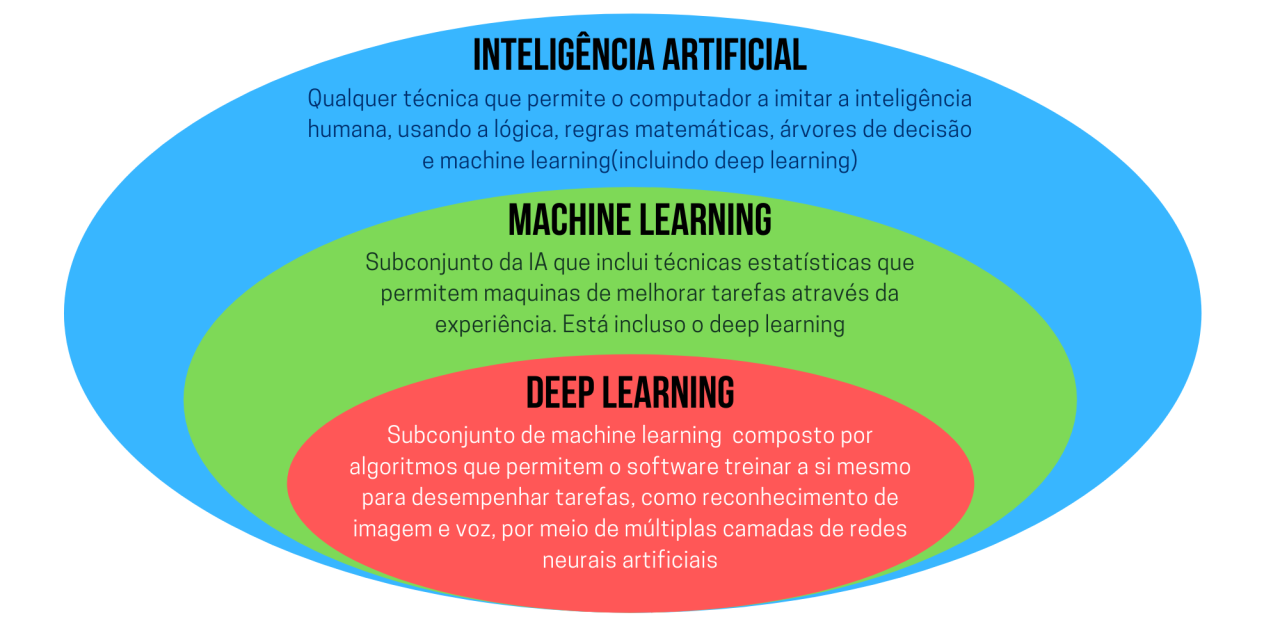
\includegraphics[width=1.11\textwidth]{figs/Machine_Learning_IA.png}
    \end{figure}
\end{frame}

% Slide 2: História e Motivação
\begin{frame}{História e Motivação}
  \begin{itemize}
    \item O conceito de Machine Learning tem raízes nos campos de estatística, ciência da computação e neurociência.
    \item Nos últimos anos, avanços em poder computacional e volume de dados aceleraram o desenvolvimento de técnicas de ML.
    \item Motivação principal: permitir que máquinas processem grandes volumes de dados e aprendam automaticamente padrões úteis.
  \end{itemize}
\end{frame}

% Slide 3: Principais Aplicações
\begin{frame}{Principais Aplicações}
  \begin{itemize}
    \item Detecção de fraudes financeiras.
    \item Reconhecimento de imagem e fala.
    \item Sistemas de recomendação (ex.: Netflix, Amazon).
    \item Diagnóstico e previsão em saúde.
    \item Carros autônomos.
  \end{itemize}
\end{frame}
% Slide 4: Formas de Aprendizado (Seção 19.1)
\begin{frame}{Formas de Aprendizado}
  \begin{itemize}
    \item Aprendizado Supervisionado:
    \begin{itemize}
        \item O algoritmo é treinado com dados rotulados.
        \item Exemplo: Classificação de imagens em categorias como "gato" ou "cachorro".
    \end{itemize}
    \item Aprendizado Não Supervisionado:
    \begin{itemize}
        \item Não há rótulos; o algoritmo identifica padrões nos dados.
        \item Exemplo: Agrupamento de clientes em segmentos de mercado.
    \end{itemize}
    \item Aprendizado por Reforço:
    \begin{itemize}
        \item O agente aprende interagindo com o ambiente e recebendo recompensas ou penalidades.
        \item Exemplo: Treinar um robô para jogar xadrez.
    \end{itemize}
  \end{itemize}
\end{frame}

\begin{frame}{Formas de Aprendizado}
\begin{figure}[h]
         \centering
         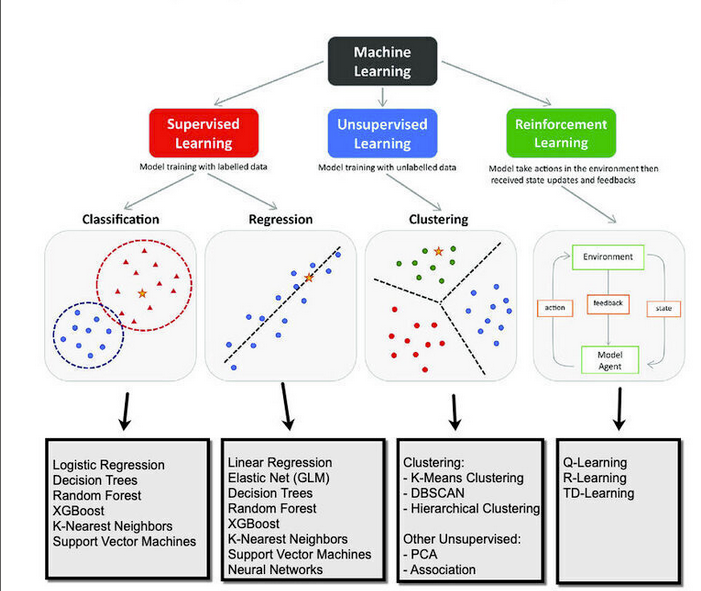
\includegraphics[width=0.7\textwidth]{figs/Machine_Learning_Types.png}
    \end{figure}
\end{frame}

% Slide 5: Detalhes Adicionais sobre Aprendizado
\begin{frame}{Detalhes sobre Formas de Aprendizado}
  \begin{itemize}
    \item Supervisionado:
    \begin{itemize}
        \item Tarefas comuns: regressão e classificação.
        \item Requer um conjunto grande de dados rotulados.
    \end{itemize}
    \item Não Supervisionado:
    \begin{itemize}
        \item Focado em identificar estrutura ou padrões ocultos.
        \item Métodos: clustering, redução de dimensionalidade.
    \end{itemize}
    \item Reforço:
    \begin{itemize}
        \item Baseado na ideia de explorar e explorar (explore vs. exploit).
        \item Utilizado em controle robótico e jogos.
    \end{itemize}
  \end{itemize}
\end{frame}

\section{Supervised Learning}
\subsection{Conceitos Fundamentais}
\begin{frame}
\centering
\Huge
\textbf{Supervised\\ Learning}
\end{frame}

% Slide 2: Introdução ao Aprendizado Supervisionado
\begin{frame}{Aprendizado Supervisionado}
    \begin{itemize}
        \item \textbf{Definição:} Um tipo de aprendizado de máquina onde o modelo é treinado utilizando dados rotulados.
        \item \textbf{Objetivo:} Aprender um mapeamento de entradas (características) para saídas (rótulos).
        \item \textbf{Aplicações:}
        \begin{itemize}
            \item Classificação de imagens
            \item Detecção de spam
            \item Análises preditivas
        \end{itemize}
    \end{itemize}
\end{frame}

% Slide 3: Componentes Chave do Aprendizado Supervisionado
\begin{frame}{Componentes Chave}
    \begin{itemize}
        \item \textbf{Conjunto de Dados:}
        \begin{itemize}
            \item Características de entrada (\textit{X})
            \item Rótulos ou valores-alvo (\textit{y})
        \end{itemize}
        \item \textbf{Modelo:}
        \begin{itemize}
            \item Função que mapeia \textit{X} para \textit{y}
        \end{itemize}
        \item \textbf{Treinamento:}
        \begin{itemize}
            \item Processo de ajuste dos parâmetros do modelo para minimizar o erro.
        \end{itemize}
        \item \textbf{Avaliação:}
        \begin{itemize}
            \item Avaliar o desempenho do modelo usando métricas como acurácia, precisão, etc.
        \end{itemize}
    \end{itemize}
\end{frame}

% Slide 4: Fluxo de Trabalho do Aprendizado Supervisionado
\begin{frame}{Fluxo de Trabalho}
    \begin{enumerate}
        \item Coletar e pré-processar dados rotulados.
        \item Dividir os dados em conjuntos de treinamento e teste.
        \item Treinar o modelo no conjunto de treinamento.
        \item Avaliar o modelo no conjunto de teste.
        \item Ajustar o modelo conforme necessário.
    \end{enumerate}

\end{frame}

\begin{frame}
      \centering
    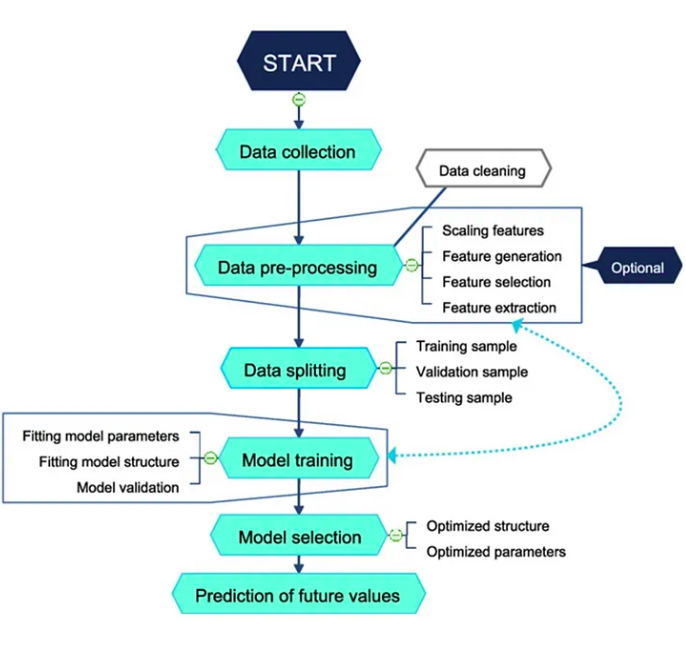
\includegraphics[width=0.8\textwidth]{figs/fluxoSupervisedLearning.png} % Substituir por imagem do livro, se disponível
\end{frame}

% Slide 5: Tipos de Aprendizado Supervisionado
\begin{frame}{Tipos de Aprendizado Supervisionado}
    \begin{itemize}
        \item \textbf{Classificação:}
        \begin{itemize}
            \item As saídas são rótulos discretos (ex.: spam ou não spam).
        \end{itemize}
        \item \textbf{Regressão:}
        \begin{itemize}
            \item As saídas são valores contínuos (ex.: preços de imóveis).
        \end{itemize}
    \end{itemize}
        \centering
    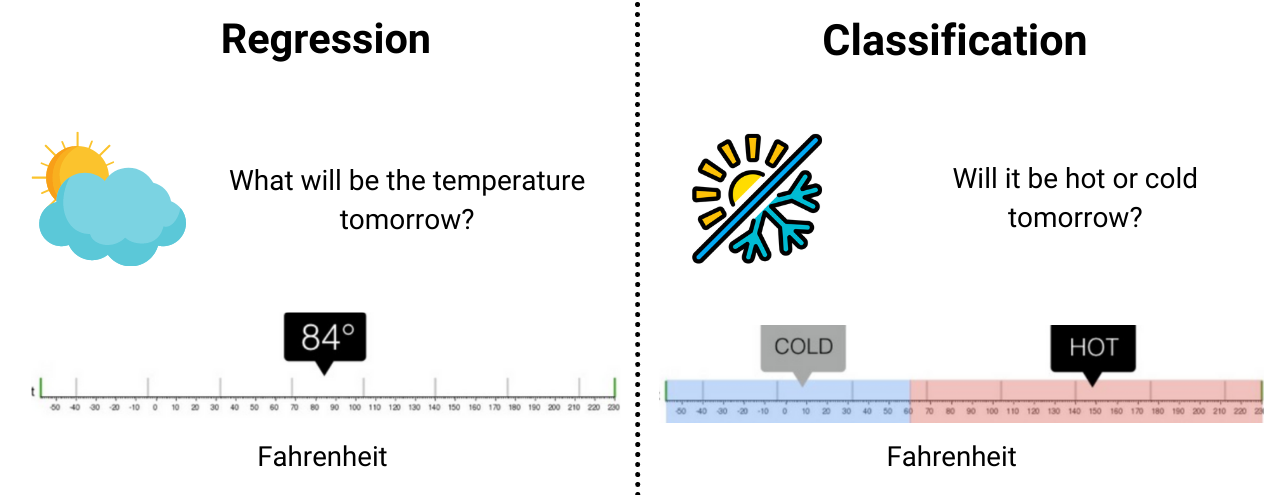
\includegraphics[width=0.8\textwidth]{figs/classificao_regressao.png} % Substituir por imagem do livro, se disponível
\end{frame}

% Slide 6: Underfitting e Overfitting
\begin{frame}{Underfitting e Overfitting}
    \begin{itemize}
        \item \textbf{Underfitting:}
        \begin{itemize}
            \item O modelo é muito simples para capturar a complexidade dos dados.
            \item Características principais:
            \begin{itemize}
                \item Alta taxa de erro tanto nos dados de treinamento quanto nos de teste.
                \item Modelo insuficiente para aprender os padrões subjacentes.
            \end{itemize}
            \item Exemplo: Ajustar uma linha reta em um conjunto de dados não linear.
        \end{itemize}

    \end{itemize}
\end{frame}


\begin{frame}{Underfitting e Overfitting}
    \begin{itemize}
        \item \textbf{Overfitting:}
        \begin{itemize}
            \item O modelo é excessivamente complexo e captura ruído dos dados de treinamento.
            \item Características principais:
            \begin{itemize}
                \item Baixa taxa de erro nos dados de treinamento, mas alta nos dados de teste.
                \item Modelo foca em detalhes irrelevantes, reduzindo a generalização.
            \end{itemize}
            \item Exemplo: Ajustar um polinômio de alta ordem em um conjunto pequeno de dados.
        \end{itemize}
    \end{itemize}
\end{frame}

\begin{frame}{Underfitting e Overfitting}
    \centering
    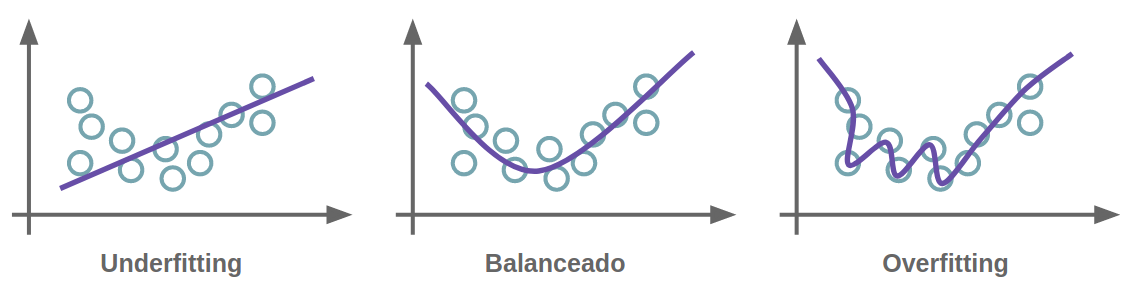
\includegraphics[width=1\textwidth]{figs/Underfitting_e_overfitting.png} % Substituir por imagem do livro, se disponível
\end{frame}
% Slide 7: Importância de Evitar Underfitting e Overfitting
\begin{frame}{Importância de Evitar}
    \begin{itemize}
        \item O objetivo do aprendizado supervisionado é construir um modelo que generalize bem para novos dados.
        \item Estratégias para evitar underfitting e overfitting:
        \begin{itemize}
            \item Escolher a complexidade adequada do modelo.
            \item Utilizar validação cruzada para avaliar o desempenho do modelo.
            \item Aplicar regularização para reduzir a complexidade do modelo.
            \item Obter mais dados de treinamento de qualidade.
        \end{itemize}
    \end{itemize}
\end{frame}



\section{Orientações para um Projeto de ML}

\subsection{Reflita sobre o problema e observe o quadro geral}
\begin{frame}{1. Reflita sobre o problema e observe o quadro geral}
    \begin{itemize}
        \item Defina o objetivo do ponto de vista do negócio.
        \item Como sua solução será usada?
        \item Quais são as soluções alternativas atuais?
        \item Como enquadrar o problema (supervisionado/não supervisionado, online/offline)?
        \item Como o desempenho deve ser medido?
        \item A medida de desempenho está alinhada com o objetivo do negócio?
        \item Qual seria o desempenho mínimo necessário?
        \item O que são problemas comparáveis? Reutilize experiências ou ferramentas.
        \item A experiência humana está disponível?
        \item Como você resolveria o problema manualmente?
        \item Liste e verifique as suposições feitas.
    \end{itemize}
\end{frame}

\subsection{Obtenha os dados}
\begin{frame}{2. Obtenha os dados}
    \begin{itemize}
        \item Liste os dados necessários e a quantidade.
        \item Encontre e documente onde obter os dados.
        \item Verifique o espaço necessário para armazenamento.
        \item Verifique as obrigações legais e obtenha autorizações.
        \item Crie um espaço de trabalho com armazenamento suficiente.
        \item Certifique-se de que informações confidenciais sejam protegidas.
        \item Verifique o tamanho e o tipo dos dados (série temporal, geográfico, etc.).
        \item Separe um conjunto de teste e não o utilize durante a exploração.
    \end{itemize}
\end{frame}

\subsection{Explore os dados para obter insights}
\begin{frame}{3. Explore os dados para obter insights}
    \begin{itemize}
        \item Crie uma cópia dos dados para exploração.
        \item Use um Notebook Jupyter para documentar a exploração.
        \item Estude cada atributo:
            \begin{itemize}
                \item Nome, tipo, \% de valores ausentes, ruído, utilidade, distribuição.
            \end{itemize}
        \item Para tarefas supervisionadas, identifique o(s) atributo(s) alvo.
        \item Visualize os dados.
        \item Estude correlações entre atributos.
        \item Identifique transformações promissoras.
        \item Documente o que foi aprendido.
    \end{itemize}
\end{frame}

\subsection{Prepare os dados}
\begin{frame}{4. Prepare os dados}
    \begin{itemize}
        \item Trabalhe em cópias dos dados (mantenha o original intacto).
        \item Grave funções para todas as transformações de dados.
        \item Limpeza de dados:
            \begin{itemize}
                \item Corrija ou remova outliers.
                \item Preencha valores ausentes (zero, média, mediana) ou descarte linhas/colunas.
            \end{itemize}
        \item Seleção de atributos:
            \begin{itemize}
                \item Descarte atributos que não fornecem informações úteis.
            \end{itemize}
        \item Engenharia de atributos:
            \begin{itemize}
                \item Decomponha atributos (categóricos, data/hora).
                \item Adicione transformações promissoras (log, sqrt, etc.).
                \item Agregue atributos em novos atributos promissores.
            \end{itemize}
        \item Escalonamento de atributos:
            \begin{itemize}
                \item Padronize ou normalize atributos.
            \end{itemize}
    \end{itemize}
\end{frame}

\subsection{Explore muitos modelos e selecione os melhores}
\begin{frame}{5. Explore muitos modelos e selecione os melhores}
    \begin{itemize}
        \item Treine modelos de diferentes categorias (linear, SVM, Random Forest, Redes Neurais, etc.).
        \item Avalie e compare o desempenho usando validação cruzada.
        \item Analise as variáveis mais significativas para cada algoritmo.
        \item Analise os tipos de erros cometidos pelos modelos.
        \item Execute uma rodada rápida de seleção e engenharia de atributos.
        \item Liste os três a cinco modelos mais promissores.
    \end{itemize}
\end{frame}

\subsection{Ajuste seus modelos e combine-os}
\begin{frame}{6. Ajuste seus modelos e combine-os}
    \begin{itemize}
        \item Ajuste os hiperparâmetros usando validação cruzada.
        \item Trate as transformações de dados como hiperparâmetros.
        \item Prefira busca aleatória em vez de busca em grade.
        \item Experimente métodos de ensemble (combinação de modelos).
        \item \textbf{Atenção}: Não ajuste o modelo após medir o erro de generalização.
    \end{itemize}
\end{frame}

\subsection{Apresente sua solução}
\begin{frame}{7. Apresente sua solução}
    \begin{itemize}
        \item Documente o que foi feito.
        \item Crie uma boa apresentação, destacando o quadro geral.
        \item Explique por que a solução atinge o objetivo de negócios.
        \item Apresente pontos interessantes observados durante o projeto.
        \item Liste suposições e limitações do sistema.
        \item Use visualizações para comunicar descobertas importantes.
    \end{itemize}
\end{frame}

\subsection{Coloque seu projeto em produção}
\begin{frame}{8. Coloque seu projeto em produção}
    \begin{itemize}
        \item Prepare a solução para produção (conecte-a às entradas de dados, escreva testes).
        \item Escreva código de monitoramento para verificar o desempenho ao vivo.
        \item Monitore a qualidade das entradas (sensores defeituosos, dados obsoletos).
        \item Treine modelos regularmente com dados atualizados (automatize o máximo possível).
    \end{itemize}
\end{frame}

\begin{frame}{Como funciona na prática}
    \begin{itemize}
        \item \url{github.com/eltonsarmanho/InteligenciaArtificial}
        \begin{itemize}
         \item Dataset
         \item k-Nearest Neighbors
         \item Decision Tree
         \item Random Forest
         \item NAIVE BAYES
         \item ENSEMBLE LEARNER
         \item SVM
        \end{itemize}
\item  Grid Search
\item Cross-Validation
\item Curva de Aprendizado
    \end{itemize}
\end{frame}

\section{Model Selection e Optimization}
\begin{frame}
\centering
\Huge
\textbf{Model Selection\\ Optimization}
\end{frame}

\begin{frame}{Seleção de Modelos (Model Selection)}
    \textbf{Objetivo:} Escolher o melhor modelo ou espaço de hipóteses para um problema de aprendizado de máquina.

    \begin{itemize}
        \item \textbf{Model Selection:} Escolha de um espaço de hipóteses (e.g., árvores de decisão, redes neurais, etc.).
        \item \textbf{Otimização:} Encontrar a melhor hipótese dentro do espaço escolhido.
    \end{itemize}

    \textbf{Desafio:} Equilibrar underfitting e overfitting.
\end{frame}

% Slide: Seleção e Otimização de Modelos
\begin{frame}{Model Selection}
    \textbf{Objetivo da seleção de modelos:}
    \begin{itemize}
        \item Identificar o modelo que melhor generaliza para dados não vistos.
    \end{itemize}

    \vspace{0.5cm}
    \textbf{Etapas principais:}
    \begin{enumerate}
        \item \textbf{Divisão dos dados:}
        \begin{itemize}
            \item \textit{Training set}: para ajustar os parâmetros do modelo.
            \item \textit{Validation set}: para ajustar hiperparâmetros.
            \item \textit{Test set}: para avaliar a performance final.
        \end{itemize}
        \item \textbf{Validação cruzada (Cross-validation):}
        \begin{itemize}
            \item Técnica para maximizar o uso dos dados disponíveis e reduzir viés.
        \end{itemize}
        \item \textbf{Escolha de métricas:}
        \begin{itemize}
            \item Exemplo: Acurácia, precisão, recall, F1-score para classificação.
        \end{itemize}
    \end{enumerate}
\end{frame}

% Slide: Validação Cruzada
\begin{frame}{Cross-validation}
    \textbf{Definição:}
    \begin{itemize}
        \item Divide os dados em \textit{k} subconjuntos (\textit{folds}).
        \item Treina e avalia o modelo \textit{k} vezes, cada vez utilizando um fold diferente como validação.
    \end{itemize}

    \vspace{0.5cm}
    \textbf{Vantagens:}
    \begin{itemize}
        \item Usa os dados de forma eficiente.
        \item Reduz a variação associada à divisão específica de dados.
    \end{itemize}
\end{frame}

\begin{frame}{Cross-validation}
    \begin{center}
        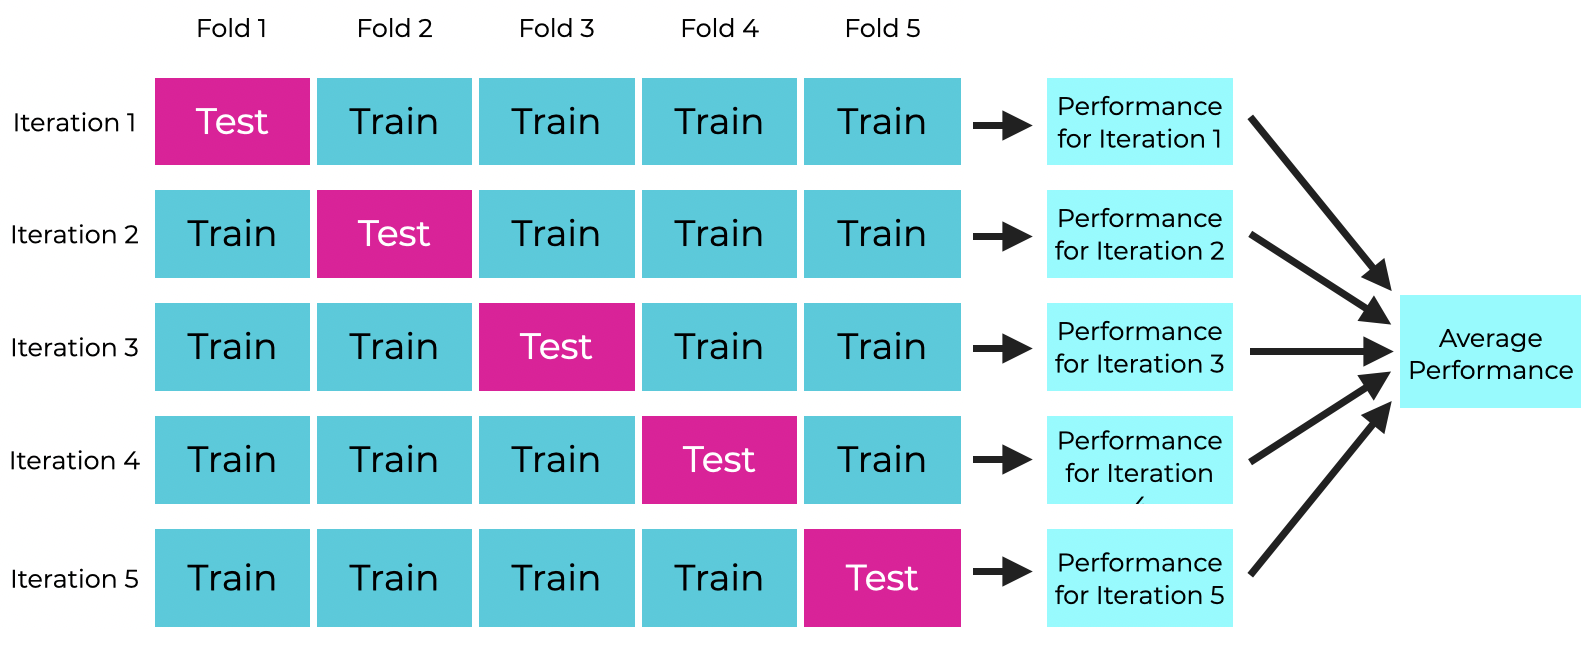
\includegraphics[width=1\textwidth]{figs/cross_validation.png}
    \end{center}
\end{frame}
\begin{frame}{Curva de Aprendizado}
    \begin{itemize}
        \item \textbf{Definição:} Representação gráfica que mostra como o desempenho de um modelo muda com o aumento de dados de treinamento.
        \item \textbf{Componentes:}
        \begin{itemize}
            \item \textbf{Erro de treinamento:} Diminui à medida que o modelo aprende melhor os padrões dos dados.
            \item \textbf{Erro de validação:} Inicialmente diminui, mas pode aumentar devido ao \textit{overfitting}.
        \end{itemize}
        \item \textbf{Objetivo:} Utilizar a curva para identificar problemas como \textit{underfitting} (alta taxa de erro) ou \textit{overfitting} (grande diferença entre erros de treinamento e validação).
    \end{itemize}

\end{frame}
\begin{frame}{Exemplo de Curva de Aprendizado}
    \begin{figure}[ht]
        \centering
        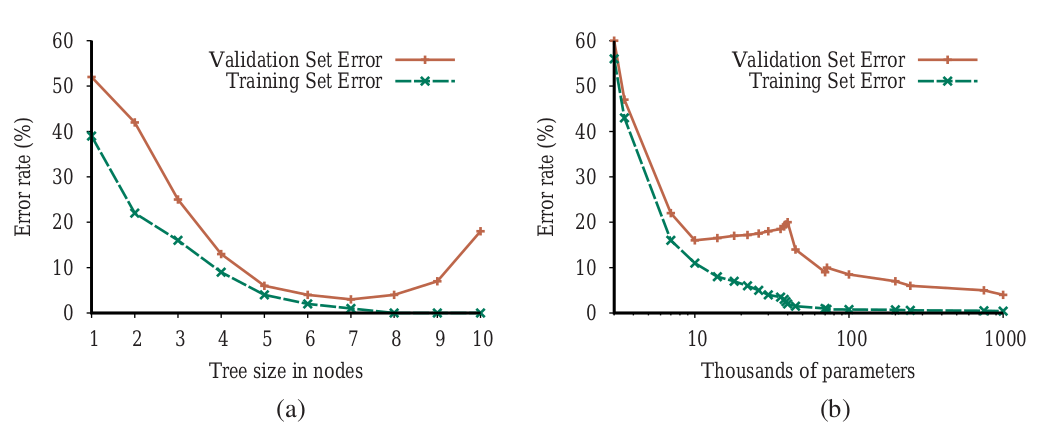
\includegraphics[width=0.85\textwidth]{figs/figura_19_9.png}

    \end{figure}

    \textbf{Curva de Aprendizado:} Mostra o erro no conjunto de treinamento e validação em função do tamanho do conjunto de treinamento.
    \begin{itemize}
        \item \textbf{Underfitting:} Erro alto em ambos os conjuntos.
        \item \textbf{Overfitting:} Erro baixo no treinamento, mas alto na validação.
    \end{itemize}
\end{frame}

% Slide: Hiperparâmetros
\begin{frame}{Hyperparameter Tuning}
    \textbf{Definição:}
    \begin{itemize}
        \item Parâmetros que não são aprendidos diretamente pelo modelo.
        \item Exemplo: número de árvores em uma floresta aleatória.
    \end{itemize}

    \vspace{0.5cm}
    \textbf{Técnicas comuns:}
    \begin{itemize}
        \item \textit{Grid search}: Busca exaustiva por combinações de hiperparâmetros.
        \item \textit{Random search}: Seleção aleatória de combinações.
        \item \textit{Bayesian optimization}: Abordagem probabilística para encontrar a melhor configuração.
    \end{itemize}
\end{frame}

\section{Matrix de Confusão}
\begin{frame}
\centering
\Huge
\textbf{Matrix \\de\\ Confusão}
\end{frame}
\begin{frame}{O que é uma Matriz de Confusão?}
    \textbf{Matriz de Confusão:}
    \begin{itemize}
        \item Ferramenta para avaliar o desempenho de modelos de classificação.
        \item Compara as previsões do modelo com os valores reais (rótulos verdadeiros).
        \item Útil para problemas de classificação binária ou multiclasse.
    \end{itemize}

    \textbf{Estrutura Básica:}
    \begin{table}[]
        \begin{tabular}{|c|c|c|}
            \hline
            & \textbf{Previsto Positivo} & \textbf{Previsto Negativo} \\ \hline
            \textbf{Real Positivo} & Verdadeiro Positivo (VP) & Falso Negativo (FN) \\ \hline
            \textbf{Real Negativo} & Falso Positivo (FP) & Verdadeiro Negativo (VN) \\ \hline
        \end{tabular}
    \end{table}
\end{frame}

\begin{frame}{Exemplo de Matriz de Confusão}
    \textbf{Cenário:} Classificação de e-mails como \textbf{spam} ou \textbf{não spam}.

    \begin{table}[]
        \begin{tabular}{|c|c|c|}
            \hline
            & \textbf{Previsto Spam} & \textbf{Previsto Não Spam} \\ \hline
            \textbf{Real Spam} & 50 (VP) & 10 (FN) \\ \hline
            \textbf{Real Não Spam} & 5 (FP) & 100 (VN) \\ \hline
        \end{tabular}
    \end{table}

    \textbf{Legenda:}
    \begin{itemize}
        \item \textbf{VP (Verdadeiro Positivo):} E-mails corretamente classificados como spam.
        \item \textbf{FN (Falso Negativo):} E-mails spam classificados como não spam.
        \item \textbf{FP (Falso Positivo):} E-mails não spam classificados como spam.
        \item \textbf{VN (Verdadeiro Negativo):} E-mails corretamente classificados como não spam.
    \end{itemize}
\end{frame}

\begin{frame}{Métricas Derivadas da Matriz de Confusão}
\footnotesize
    \textbf{1. Acurácia (Accuracy):}
    \[
    \text{Acurácia} = \frac{VP + VN}{VP + FP + FN + VN}
    \]
    \textbf{Exemplo:} \(\frac{50 + 100}{50 + 5 + 10 + 100} = \frac{150}{165} \approx 90.9\%\).

    \textbf{2. Precisão (Precision):}
    \[
    \text{Precisão} = \frac{VP}{VP + FP}
    \]
    \textbf{Exemplo:} \(\frac{50}{50 + 5} = \frac{50}{55} \approx 90.9\%\).

    \textbf{3. Recall (Sensibilidade):}
    \[
    \text{Recall} = \frac{VP}{VP + FN}
    \]
    \textbf{Exemplo:} \(\frac{50}{50 + 10} = \frac{50}{60} \approx 83.3\%\).

    \textbf{4. F1-Score:}
    \[
    \text{F1-Score} = 2 \cdot \frac{\text{Precisão} \cdot \text{Recall}}{\text{Precisão} + \text{Recall}}
    \]
    \textbf{Exemplo:} \(2 \cdot \frac{0.909 \cdot 0.833}{0.909 + 0.833} \approx 0.869\).
\end{frame}

\begin{frame}{Interpretação da Matriz de Confusão}
    \textbf{1. Underfitting (Subajuste):}
    \begin{itemize}
        \item Alto erro tanto no treinamento quanto na validação.
        \item Modelo muito simples para capturar os padrões dos dados.
    \end{itemize}

    \textbf{2. Overfitting (Sobreajuste):}
    \begin{itemize}
        \item Baixo erro no treinamento, mas alto erro na validação.
        \item Modelo se ajusta demais aos dados de treinamento e não generaliza bem.
    \end{itemize}

    \textbf{3. Bom Ajuste:}
    \begin{itemize}
        \item Baixo erro tanto no treinamento quanto na validação.
        \item Modelo generaliza bem para novos dados.
    \end{itemize}
\end{frame}

\begin{frame}{Matriz de Confusão para Classificação Multiclasse}
    \textbf{Exemplo:} Problema com três classes (\textbf{A}, \textbf{B}, \textbf{C}).

    \begin{table}[]
        \begin{tabular}{|c|c|c|c|}
            \hline
            & \textbf{Previsto A} & \textbf{Previsto B} & \textbf{Previsto C} \\ \hline
            \textbf{Real A} & VP\_A & FN\_A→B & FN\_A→C \\ \hline
            \textbf{Real B} & FN\_B→A & VP\_B & FN\_B→C \\ \hline
            \textbf{Real C} & FN\_C→A & FN\_C→B & VP\_C \\ \hline
        \end{tabular}
    \end{table}

    \textbf{Legenda:}
    \begin{itemize}
        \item \textbf{VP\_X:} Verdadeiros positivos para a classe X.
        \item \textbf{FN\_X→Y:} Falsos negativos onde a classe real era X, mas foi prevista como Y.
    \end{itemize}
\end{frame}


\begin{frame}{Matriz de Confusão para Classificação Multiclasse}
   \begin{center}
        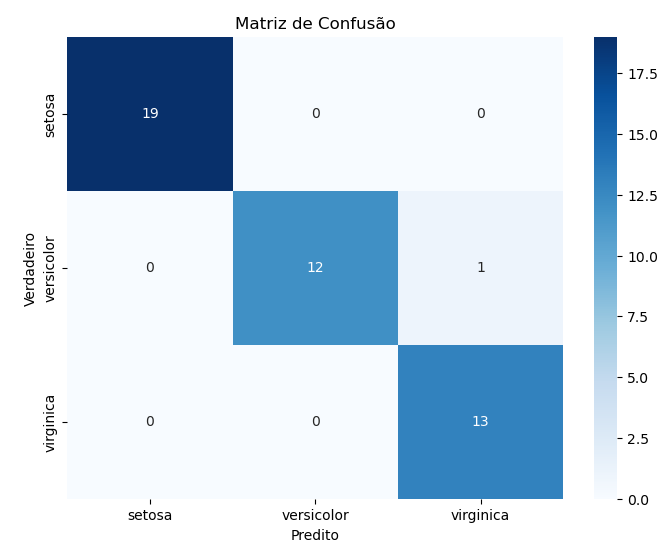
\includegraphics[width=0.75\textwidth]{figs/matrix.png}
    \end{center}
\end{frame}

\begin{frame}{Matriz de Confusão para Classificação Multiclasse}
   \begin{center}
        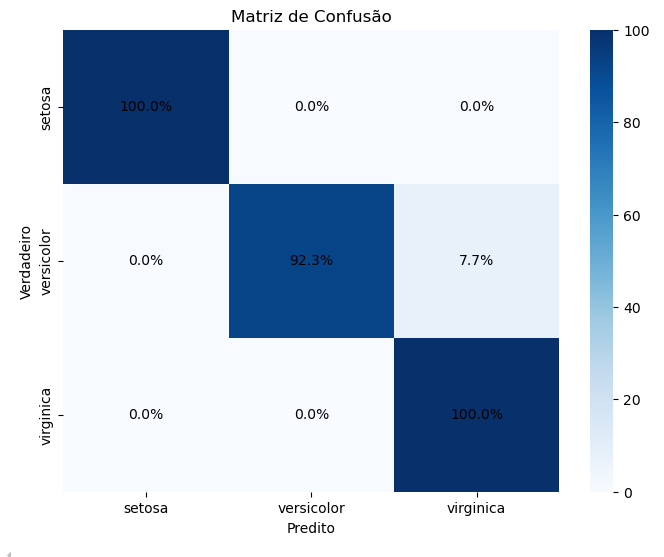
\includegraphics[width=0.75\textwidth]{figs/matrix2.png}
    \end{center}
\end{frame}

\begin{frame}{Quando Usar a Matriz de Confusão?}
    \textbf{Aplicações:}
    \begin{itemize}
        \item Avaliação de modelos de classificação.
        \item Identificação de desbalanceamento de classes.
        \item Ajuste de limiares de decisão para equilibrar precisão e recall.
    \end{itemize}


\end{frame}

\section{Fundamentos de Regressão}
\begin{frame}
\centering
\Huge
\textbf{Regressão}
\end{frame}

\begin{frame}{}
\footnotesize
  \begin{block}{Definição}
    Modelo estatístico para prever uma variável contínua \( y \) a partir de uma ou mais variáveis de entrada \( X \).
    \[
    y = \beta_0 + \beta_1 x_1 + \beta_2 x_2 + \cdots + \beta_n x_n + \varepsilon
    \]
  \end{block}

  \begin{figure}[ht]
    \centering
    \begin{tikzpicture}[scale=0.7]
      \begin{axis}[
          xlabel=\( x \),
          ylabel=\( y \),
          axis lines=left,
          scatter/classes={%
            a={mark=*, draw=black, fill=blue!50}},
          ]
        \addplot[scatter, only marks, scatter src=explicit symbolic]
        coordinates {
          (1, 2) [a] (2, 3) [a] (3, 5) [a] (4, 4) [a] (5, 6) [a]
        };
        \addplot[thick, red] {1.2*x + 0.5};
        \node at (axis cs: 3,7) {Reta de regressão};
      \end{axis}
    \end{tikzpicture}
    \caption{Exemplo de regressão linear.}
  \end{figure}
\end{frame}

\begin{frame}{Regressão vs. Classificação}
\vspace*{-1cm}
\footnotesize
  \begin{table}[h!]
    \centering
    \begin{tabular}{|l|l|l|}
      \hline
      \textbf{Característica} & \textbf{Regressão} & \textbf{Classificação} \\
      \hline
      Saída & Contínua (\( \mathbb{R} \)) & Discreta (rótulos) \\
      Exemplo & Preço de imóveis & Diagnóstico médico (doente/saudável) \\
      Métricas & MSE, \( R^2 \) & Acurácia, F1-Score \\
      \hline
    \end{tabular}
  \end{table}


\end{frame}

\begin{frame}{Variáveis Independentes vs. Dependentes}
  \begin{columns}
    \column{0.5\textwidth}
    \begin{block}{Formulação Matemática}
      \[
      \mathbf{y} = \mathbf{X}\boldsymbol{\beta} + \boldsymbol{\varepsilon}
      \]
      Onde:
      \begin{itemize}
        \item \( \mathbf{X} \in \mathbb{R}^{n \times p} \): Matriz de features
        \item \( \boldsymbol{\beta} \in \mathbb{R}^p \): Vetor de coeficientes
        \item \( \boldsymbol{\varepsilon} \in \mathbb{R}^n \): Erro aleatório
      \end{itemize}
    \end{block}

    \column{0.5\textwidth}
    \begin{tikzpicture}[
        node distance=1cm,
        var/.style={rectangle, draw=blue!50, fill=blue!10, minimum width=2cm}
      ]
      \node (X) [var] {Variáveis Independentes (\( X \))};
      \node (model) [below=of X, ellipse, draw=red!50, fill=red!10] {Modelo (\( f \))};
      \node (y) [below=of model, var] {Variável Dependente (\( y \))};

      \draw[->] (X) -- (model) node[midway, right] {\( \mathbf{X}\boldsymbol{\beta} \)};
      \draw[->] (model) -- (y) node[midway, right] {\( \hat{y} \)};
    \end{tikzpicture}
  \end{columns}
\end{frame}

\subsection{Tipos de Modelos de Regressão}

\begin{frame}{Regressão Linear Simples}
\footnotesize
  \begin{block}{Definição}
    Modela a relação linear entre uma variável independente \( x \) e uma variável dependente \( y \):
    \[
    y = \beta_0 + \beta_1 x + \varepsilon
    \]
    Onde:
    \begin{itemize}
      \item \( \beta_0 \): Intercepto (valor de \( y \) quando \( x = 0 \)).
      \item \( \beta_1 \): Coeficiente angular (inclinação da reta).
      \item \( \varepsilon \): Erro aleatório.
    \end{itemize}
  \end{block}
    \centering
\vspace*{-0.1cm}
   \begin{tikzpicture}[scale=0.4]
      \begin{axis}[
          xlabel=\( x \),
          ylabel=\( y \),
          axis lines=left,
          scatter/classes={%
            a={mark=*, draw=black, fill=blue!50}},
          ]
        \addplot[scatter, only marks, scatter src=explicit symbolic]
        coordinates {
          (1, 2) [a] (2, 3) [a] (3, 5) [a] (4, 4) [a] (5, 6) [a]
        };
        \addplot[thick, red] {1.2*x + 0.5};
        \node at (axis cs: 3,7) {Reta de regressão};
      \end{axis}
    \end{tikzpicture}
\end{frame}

\begin{frame}{Regressão Linear Múltipla}
\footnotesize

  \begin{block}{Definição}
    Estende a regressão linear para múltiplas variáveis independentes:
    \[
    y = \beta_0 + \beta_1 x_1 + \beta_2 x_2 + \cdots + \beta_n x_n + \varepsilon
    \]
    Em forma matricial:
    \[
    \mathbf{y} = \mathbf{X}\boldsymbol{\beta} + \boldsymbol{\varepsilon}
    \]
    Onde:
    \begin{itemize}
      \item \( \mathbf{X} \): Matriz de features (\( n \times p \)).
      \item \( \boldsymbol{\beta} \): Vetor de coeficientes (\( p \times 1 \)).
    \end{itemize}
  \end{block}

  \begin{tikzpicture}[overlay, remember picture]
    \node[anchor=south east, xshift=-20pt, yshift=45pt] at (current page.south east) {
      \begin{tikzpicture}[scale=0.5]
        \draw[->] (-1,0) -- (3,0) node[right] {\( x_1 \)};
        \draw[->] (0,-1) -- (0,3) node[above] {\( x_2 \)};
        \draw[->] (2,2) -- (2.5,2.5) node[right] {\( y \)};
        \foreach \x/\y in {0.5/1, 1/1.5, 2/2.5, 1.5/3}
          \fill[blue] (\x,\y) circle (2pt);
      \end{tikzpicture}
    };
  \end{tikzpicture}
\end{frame}

\begin{frame}{Regressão Polinomial}
\footnotesize
  \begin{block}{Definição}
    Modela relações não lineares usando polinômios:
    \[
    y = \beta_0 + \beta_1 x + \beta_2 x^2 + \cdots + \beta_n x^n + \varepsilon
    \]
    Exemplo: \( y = \beta_0 + \beta_1 x + \beta_2 x^2 \).
  \end{block}

  \begin{figure}[ht]
    \centering
    \begin{tikzpicture}[scale=0.6]
      \begin{axis}[
          xlabel=\( x \),
          ylabel=\( y \),
          axis lines=left,
          scatter/classes={%
            a={mark=*, draw=black, fill=blue!50}},
          ]
        \addplot[scatter, only marks, scatter src=explicit symbolic]
        coordinates {
          (1, 2) [a] (2, 3) [a] (3, 5) [a] (4, 4) [a] (5, 6) [a]
        };
        \addplot[thick, red] {0.5*x^2 - 1.5*x + 3};
        \node at (axis cs: 3,7) {Curva de regressão polinomial};
      \end{axis}
    \end{tikzpicture}

  \end{figure}
\end{frame}

\begin{frame}{Regressão Regularizada}
\footnotesize
  \begin{block}{Objetivo}
    Penalizar coeficientes grandes para evitar overfitting:
    \begin{itemize}
      \item Ridge (L2):
        \[
        \text{Minimizar } \|\mathbf{y} - \mathbf{X}\boldsymbol{\beta}\|^2 + \lambda \|\boldsymbol{\beta}\|^2
        \]
      \item Lasso (L1):
        \[
        \text{Minimizar } \|\mathbf{y} - \mathbf{X}\boldsymbol{\beta}\|^2 + \lambda \|\boldsymbol{\beta}\|_1
        \]
      \item Elastic Net:
        \[
        \text{Minimizar } \|\mathbf{y} - \mathbf{X}\boldsymbol{\beta}\|^2 + \lambda_1 \|\boldsymbol{\beta}\|_1 + \lambda_2 \|\boldsymbol{\beta}\|^2
        \]
    \end{itemize}
  \end{block}

\end{frame}

\begin{frame}{Regressão Logística (Contexto de Regressão)}
\footnotesize
  \begin{block}{Definição}
    Usada para problemas de classificação binária, mas fundamentada em regressão:
    \[
    P(y=1 | \mathbf{x}) = \frac{1}{1 + e^{-(\beta_0 + \beta_1 x_1 + \cdots + \beta_n x_n)}}
    \]
    Onde:
    \begin{itemize}
      \item \( P(y=1 | \mathbf{x}) \): Probabilidade de \( y = 1 \).
      \item Função logística: \( \sigma(z) = \frac{1}{1 + e^{-z}} \).
    \end{itemize}
  \end{block}

  \begin{figure}[ht]
    \centering
    \begin{tikzpicture}[scale=0.4]
      \begin{axis}[
          xlabel=\( z \),
          ylabel=\( \sigma(z) \),
          axis lines=left,
          ]
        \addplot[thick, red, domain=-5:5] {1/(1+exp(-x))};
      \end{axis}
    \end{tikzpicture}

  \end{figure}
\end{frame}

\subsection{Métricas de Avaliação}

% Slide sobre MSE
\begin{frame}{Erro Quadrático Médio (MSE)}
    \textbf{Definição:}
    O Erro Quadrático Médio é uma métrica que mede a média dos erros ao quadrado entre os valores reais ($y_i$) e os valores preditos ($\hat{y}_i$):
    \begin{equation}
        \text{MSE} = \frac{1}{n} \sum_{i=1}^{n} (y_i - \hat{y}_i)^2
    \end{equation}
    \textbf{Interpretação:} Quanto menor o MSE, melhor a performance do modelo.

    \vspace{0.3cm}
    \textbf{Visualização:}
    \begin{tikzpicture}[scale=0.4]
        \draw[->] (0,0) -- (6,0) node[right] {$\hat{y}_i$};
        \draw[->] (0,0) -- (0,4) node[above] {$y_i$};
        \draw[dashed, red] (1,1) -- (1,2.5) node[midway, left] {$(y_i - \hat{y}_i)^2$};
        \draw[fill] (1,1) circle (2pt) node[below right] {$\hat{y}_i$};
        \draw[fill] (1,2.5) circle (2pt) node[above right] {$y_i$};
    \end{tikzpicture}
\end{frame}


% Slide sobre RMSE
\begin{frame}{Raiz do Erro Quadrático Médio (RMSE)}
    \textbf{Definição:}
    A Raiz do Erro Quadrático Médio é simplesmente a raiz quadrada do MSE:
    \begin{equation}
        \text{RMSE} = \sqrt{\text{MSE}} = \sqrt{\frac{1}{n} \sum_{i=1}^{n} (y_i - \hat{y}_i)^2}
    \end{equation}
    \textbf{Interpretação:} É uma métrica na mesma unidade dos dados originais, tornando sua interpretação mais intuitiva.
\end{frame}

% Slide sobre MAE
\begin{frame}{Erro Absoluto Médio (MAE)}
    \textbf{Definição:}
    O Erro Absoluto Médio mede a média das diferenças absolutas entre os valores reais e preditos:
    \begin{equation}
        \text{MAE} = \frac{1}{n} \sum_{i=1}^{n} |y_i - \hat{y}_i|
    \end{equation}
    \textbf{Interpretação:} Valores menores indicam que o modelo está mais próximo dos valores reais em média.
\end{frame}

% Slide sobre R² e R² Ajustado
\begin{frame}{Coeficiente de Determinação ($R^2$) e $R^2$ Ajustado}
    \textbf{Coeficiente de Determinação ($R^2$):}
    \begin{itemize}
        \item Mede a proporção da variância explicada pelo modelo.
        \item Fórmula:
        \begin{equation}
            R^2 = 1 - \frac{\sum_{i=1}^{n} (y_i - \hat{y}_i)^2}{\sum_{i=1}^{n} (y_i - \bar{y})^2}
        \end{equation}
        \item Intervalo: $0 \leq R^2 \leq 1$ (quanto mais próximo de 1, melhor).
    \end{itemize}

    \textbf{$R^2$ Ajustado:}
    \begin{itemize}
        \item Penaliza a adição de variáveis irrelevantes ao modelo.
        \item Fórmula:
        \begin{equation}
            R^2_{\text{ajustado}} = 1 - \left(1 - R^2\right) \frac{n - 1}{n - p - 1}
        \end{equation}
        \item Onde $p$ é o número de variáveis explicativas.
    \end{itemize}
\end{frame}


\subsection{Suposições da Regressão Linear}

\begin{frame}{Linearidade}
    \textbf{Definição:}
    A relação entre a variável dependente ($y$) e a variável independente ($X$) deve ser linear.

    \vspace{0.5cm}
    \textbf{Representação Matemática:}
    \begin{equation}
        y = \beta_0 + \beta_1X + \epsilon
    \end{equation}
    Onde:
    \begin{itemize}
        \item $\beta_0$ é o intercepto;
        \item $\beta_1$ é o coeficiente angular;
        \item $\epsilon$ representa o termo de erro.
    \end{itemize}

    \hspace{3cm}
    \begin{tikzpicture}[scale=0.35]
        \draw[->] (0,0) -- (6,0) node[right] {$X$};
        \draw[->] (0,0) -- (0,4) node[above] {$y$};
        \draw[thick, blue] (0.5,1) -- (5.5,3.5) node[midway, above,xshift=60pt] {$y = \beta_0 + \beta_1X$};
        \foreach \x in {1, 2, 3, 4, 5} {
            \node[fill, circle, inner sep=1.5pt] at (\x, {0.5*\x+0.5+rand*0.3-0.15}) {};
        }
    \end{tikzpicture}
\end{frame}

% Slide sobre Independência dos Resíduos
\begin{frame}{Independência dos Resíduos}
\footnotesize
    \textbf{Definição:}
    Os resíduos ($\epsilon_i$) não devem estar correlacionados entre si.

    \vspace{0.5cm}
    \textbf{Teste Comum:} Teste de Durbin-Watson
    \begin{equation}
        DW = \frac{\sum_{i=2}^{n} (\epsilon_i - \epsilon_{i-1})^2}{\sum_{i=1}^{n} \epsilon_i^2}
    \end{equation}
    Valores próximos de 2 indicam independência.

    \vspace{0.5cm}
    \textbf{Visualização:}
    \begin{tikzpicture}[scale=0.5]
         \draw[->] (0,0) -- (6,0) node[right] {Observações};
        \draw[->] (0,-2) -- (0,2) node[above] {Resíduos ($\epsilon$)};
        \foreach \x in {1, 2, 3, 4, 5} {
            \node[fill, circle, inner sep=1.5pt] at (\x, {rand*0.5-0.25}) {};
        }
        \node at (3,-2.5) {Pontos aleatórios indicam independência};
    \end{tikzpicture}
\end{frame}

% Slide sobre Homocedasticidade
\begin{frame}{Homocedasticidade}
    \textbf{Definição:}
    A variância dos resíduos deve ser constante para todos os valores de $X$.

    \vspace{0.5cm}
    \textbf{Visualização:}
    \begin{tikzpicture}
        \draw[->] (0,0) -- (6,0) node[right] {$X$};
        \draw[->] (0,-2) -- (0,2) node[above] {Resíduos ($\epsilon$)};
        \foreach \x in {1, 2, 3, 4, 5} {
            \node[fill, circle, inner sep=1.5pt] at (\x, {rand*0.5-0.25}) {};
            \draw[dashed] (\x, -1) -- (\x, 1);
        }
    \end{tikzpicture}
\end{frame}

\begin{frame}{Homocedasticidade}
    \textbf{Interpretacao:}
    A ausência de padrões nos resíduos (em torno do eixo x) indica que o modelo atende à suposição de homocedasticidade.

    \vspace{0.5cm}
    \textbf{Visualização:}
    \begin{tikzpicture}
        \draw[->] (0,0) -- (6,0) node[right] {$X$};
        \draw[->] (0,-2) -- (0,2) node[above] {Resíduos ($\epsilon$)};
        \foreach \x in {1, 2, 3, 4, 5} {
            \node[fill, circle, inner sep=1.5pt] at (\x, {rand*0.5-0.25}) {};
            \draw[dashed] (\x, -1) -- (\x, 1);
        }
    \end{tikzpicture}
\end{frame}

\begin{frame}{Normalidade dos Resíduos}
    \textbf{Definição:}
    Os resíduos devem seguir uma distribuição aproximadamente normal.

    \vspace{0.5cm}
    \textbf{Teste Comum:} Teste de Shapiro-Wilk

    \vspace{0.5cm}
    \textbf{Visualização:}
    \begin{tikzpicture}
        \draw[->] (0,0) -- (6,0) node[right] {Resíduos ($\epsilon$)};
        \draw[->] (0,0) -- (0,3) node[above] {Frequência};
        \draw[thick, blue, domain=0:6, samples=50] plot (\x, {2*exp(-0.5*(\x-3)^2)});
    \end{tikzpicture}
\end{frame}


\begin{frame}{Ausência de Multicolinearidade}
    \textbf{Definição:}
    As variáveis independentes não devem ser altamente correlacionadas entre si.

    \vspace{0.5cm}
    \textbf{Teste Comum:} Fator de Inflacionamento da Variância (VIF)
    \begin{equation}
        \text{VIF}_j = \frac{1}{1 - R_j^2}
    \end{equation}
    Onde $R_j^2$ é o coeficiente de determinação da regressão da variável $j$ contra as demais.

    \vspace{0.5cm}
    \textbf{Interpretação:} VIF $>$ 10 indica alta multicolinearidade.
\end{frame}





\section{Redes Neurais}
\begin{frame}
\centering
\Huge
\textbf{Redes \\ Neurais}
\end{frame}

\begin{frame}
\frametitle{Objetivos da Apresentação}
\begin{itemize}
    \item Explorar as características fundamentais das Redes Neurais Artificiais (RNAs).
    \item Compreender o funcionamento básico de uma RNA.
    \item Analisar as principais arquiteturas de RNAs disponíveis.
    \item Ilustrar aplicações de RNAs em Reconhecimento de Padrões e Controle.
\end{itemize}
\end{frame}

\begin{frame}
\frametitle{Motivação Biológica}
\framesubtitle{Ideia Central}
\begin{itemize}
    \item Utilizar neurônios biológicos como modelos para neurônios artificiais.
    \item Neurônios biológicos são o elemento fundamental do sistema nervoso.
    \item Existem diversos tipos de neurônios biológicos.
\end{itemize}
\end{frame}

\begin{frame}
\frametitle{Neurônio Biológico}
\begin{itemize}
    \item O cérebro humano é relativamente lento, mas possui alto paralelismo.
    \item Cerca de $10^{11}$ neurônios, cada um operando a aproximadamente 1 KHz.
    \item Cada neurônio pode se conectar com até $10^4$ outros neurônios.
\end{itemize}
\begin{figure}
    \centering
    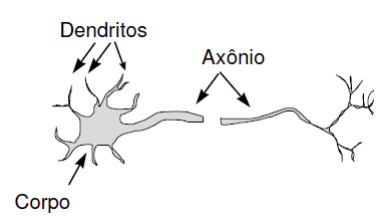
\includegraphics[width=0.5\textwidth]{figs/neuronio.png} % Substitua pelo caminho da sua imagem
    \caption{Representação de um neurônio biológico.}
    \label{fig:neuronio}
\end{figure}
\end{frame}

\begin{frame}
\frametitle{Funcionamento Simplificado de um Neurônio Biológico}
\begin{itemize}
    \item Neurônios podem estar em dois estados:
    \begin{itemize}
        \item \textbf{Ativo ou excitado}: Envia sinais para outros neurônios por meio do axônio e sinapses.
        \item \textbf{Inativo ou inibido}: Não envia sinais.
    \end{itemize}
    \item Sinapses podem ser de dois tipos:
    \begin{itemize}
        \item \textbf{Excitatorias}: Excitam o neurônio receptor.
        \item \textbf{Inibitórias}: Inibem o neurônio receptor.
    \end{itemize}
\end{itemize}
\end{frame}

\begin{frame}
\frametitle{Ativação do Neurônio}
\begin{itemize}
    \item Quando o efeito cumulativo das várias sinapses que chegam a um neurônio excede um valor limite, o neurônio dispara.
    \item O neurônio fica ativo por um período e envia um sinal para outros neurônios.
\end{itemize}
\end{frame}

\begin{frame}
\frametitle{Introdução às Redes Neurais Artificiais}
\begin{itemize}
    \item Redes neurais artificiais são modelos computacionais inspirados no funcionamento do cérebro humano.
    \item Esses modelos são amplamente utilizados em aprendizado de máquina e inteligência artificial.
    \item As redes neurais foram desenvolvidas a partir de contribuições de diversas áreas, como matemática aplicada, estatística e ciência da computação.
\end{itemize}
\end{frame}

\begin{frame}
\frametitle{Origens das Redes Neurais Artificiais}
\begin{itemize}
    \item Os primeiros estudos formais sobre redes neurais artificiais foram realizados por McCulloch e Pitts em 1943.
    \item Eles propuseram um modelo matemático para um neurônio artificial.
    \item Esse modelo era capaz de implementar operações lógicas básicas, como "E" e "OU".
\end{itemize}
\end{frame}

\begin{frame}
\frametitle{Modelo Matemático do Neurônio Artificial}
\begin{itemize}
    \item Um neurônio artificial pode ser representado por uma função \( \eta : \mathbb{R}^n \rightarrow \{0, 1\} \).
    \item A função é definida pela equação:
    \[
    \eta(x) = \chi_{\geq 0} \left[ w^T x - b \right],
    \]
    onde:
    \begin{itemize}
        \item \( w \) é o vetor de pesos,
        \item \( x \) é o vetor de entradas,
        \item \( b \) é o limiar de ativação,
        \item \( \chi_{\geq 0} \) é a função indicadora que retorna 1 se o argumento for maior ou igual a zero, e 0 caso contrário.
    \end{itemize}
\end{itemize}
\end{frame}

\begin{frame}
\frametitle{Aplicações Iniciais}
\begin{itemize}
    \item O modelo de McCulloch e Pitts demonstrou que redes neurais podem resolver problemas de lógica clássica.
    \item Essa descoberta foi um marco inicial para o desenvolvimento de sistemas de inteligência artificial.
    \item Hoje, as redes neurais são aplicadas em diversas áreas, como reconhecimento de padrões, processamento de linguagem natural e visão computacional.
\end{itemize}
\end{frame}

\begin{frame}
\frametitle{Neurônio Artificial}
\begin{itemize}
    \item Um neurônio artificial é uma função \( \eta : \mathbb{R}^n \to \mathbb{R} \).
    \item A função é definida por:
    \[
    \eta(x) = \varphi(w^T x - b),
    \]
    onde:
    \begin{itemize}
        \item \( \varphi \) é a função de ativação,
        \item \( w \) é o vetor de pesos sinápticos,
        \item \( b \) é o viés.
    \end{itemize}
\end{itemize}
\end{frame}
\subsection{Funções de Ativação}
\begin{frame}
\framesubtitle{Funções de Ativação}
\footnotesize
\begin{itemize}
    \item A função de ativação \( \varphi \) determina a saída do neurônio.

\end{itemize}
\begin{block}{Função Limiar}
\[
\chi_{\geq 0}(t) =
\begin{cases}
1, & t \geq 0, \\
0, & t < 0.
\end{cases}
\]
\end{block}
\begin{block}{Função Logística}
\[
\sigma(t) = \frac{1}{(1 + e^{-t})}.
\]
\end{block}
\begin{block}{Função ReLU}
\[
\text{relu}(t) = \max\{0, t\}.
\]
\end{block}
\end{frame}

\begin{frame}
\frametitle{Aplicações das Funções de Ativação}
\begin{itemize}
    \item A função limiar é usada em modelos binários.
    \item A função logística é comum em problemas de classificação.
    \item A função ReLU é amplamente utilizada em redes neurais profundas.
\end{itemize}
\end{frame}

\subsection{Propriedades das Redes Neurais Artificiais}
\begin{frame}
\frametitle{Propriedades das Redes Neurais Artificiais}
\begin{itemize}
    \item As redes neurais artificiais (RNAs) possuem características que as tornam poderosas para diversas aplicações.
    \item Entre as principais propriedades estão: aprendizado, generalização e abstração.
\end{itemize}
\end{frame}

\begin{frame}
\frametitle{Aprendizado}
\begin{itemize}
    \item As RNAs são capazes de modificar seu comportamento com base nos dados de entrada.
    \item Isso permite que elas produzam saídas consistentes e adaptadas ao domínio do problema.
    \item O aprendizado ocorre através da ajuste dos pesos sinápticos durante o treinamento.
\end{itemize}
\end{frame}

\begin{frame}
\frametitle{Generalização}
\begin{itemize}
    \item Após o treinamento, uma RNA pode lidar com pequenas variações nas entradas, como ruídos ou distorções.
    \item Essa capacidade de generalização é essencial para aplicações em cenários do mundo real.
    \item A generalização permite que a rede mantenha um bom desempenho mesmo com dados não vistos durante o treinamento.
\end{itemize}
\end{frame}

\subsection{Arquitetura da Rede Neural}
\begin{frame}
\frametitle{Arquitetura de Redes Neurais}
\begin{itemize}
    \item Os neurônios artificiais são as unidades básicas de processamento em uma rede neural.
    \item Uma rede neural pode ser representada como um grafo direcionado.
    \item Nesse grafo, os vértices correspondem aos neurônios e as arestas indicam conexões entre eles.
\end{itemize}
\end{frame}

\begin{frame}
\frametitle{Topologia da Rede Neural}
\begin{itemize}
    \item A estrutura do grafo é chamada de arquitetura ou topologia da rede neural.
    \item A topologia define como os neurônios estão organizados e conectados.
    \item Existem diferentes tipos de topologias, como redes neurais recorrentes e progressivas.
\end{itemize}
\end{frame}

\begin{frame}
\frametitle{Redes Neurais Recorrentes ou \textit{Feed-backward networks}}
\begin{itemize}
    \item Uma rede neural é dita recorrente quando o grafo associado contém ciclos.
    \item Isso permite que a informação flua em loops, o que é útil para modelar sequências temporais.
    \item Aplicações comuns incluem processamento de linguagem natural e previsão de séries temporais.
\end{itemize}
\end{frame}

\begin{frame}
\frametitle{Redes Neurais Recorrentes ou \textit{Feed-backward networks}}
\begin{figure}
    \centering
    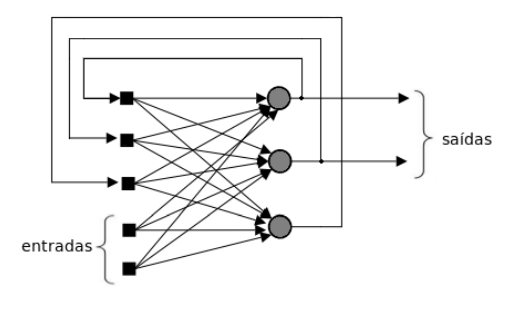
\includegraphics[width=1\textwidth]{figs/RedesRecorrentes.png} % Substitua pelo caminho da sua imagem

\end{figure}
\end{frame}



\begin{frame}
\frametitle{Redes Neurais Progressivas ou \textit{Feed-forward networks}}
\begin{itemize}
    \item Uma rede neural é progressiva quando o fluxo de informação segue em uma única direção, sem ciclos.
    \item Também conhecidas como redes feedforward, são amplamente utilizadas em tarefas de classificação e regressão.
    \item Exemplos incluem redes neurais convolucionais (CNNs) e perceptrons multicamadas.
\end{itemize}
\end{frame}

\begin{frame}
\frametitle{Redes Neurais Progressivas ou \textit{Feed-forward networks}}
\begin{figure}
    \centering
    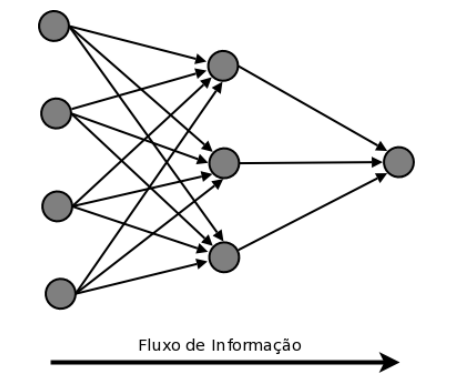
\includegraphics[width=0.8\textwidth]{figs/Feedforwardnetworks.png} % Substitua pelo caminho da sua imagem

\end{figure}
\end{frame}

\subsection{Perceptron}
\begin{frame}
\frametitle{Modelo Matemático do Perceptron}
\begin{itemize}
    \item O Perceptron é uma função \( f: \mathbb{R}^n \to \{0, 1\} \) definida por:
    \[
    f(x) = \begin{cases}
    1, & \text{se } w^T x + b \geq 0, \\
    0, & \text{caso contrário},
    \end{cases}
    \]
    onde:
    \begin{itemize}
        \item \( x \in \mathbb{R}^n \) é o vetor de entrada,
        \item \( w \in \mathbb{R}^n \) é o vetor de pesos,
        \item \( b \in \mathbb{R} \) é o viés.
    \end{itemize}
\end{itemize}
\end{frame}

\begin{frame}
\frametitle{Estrutura do Perceptron}
\begin{figure}
    \centering
    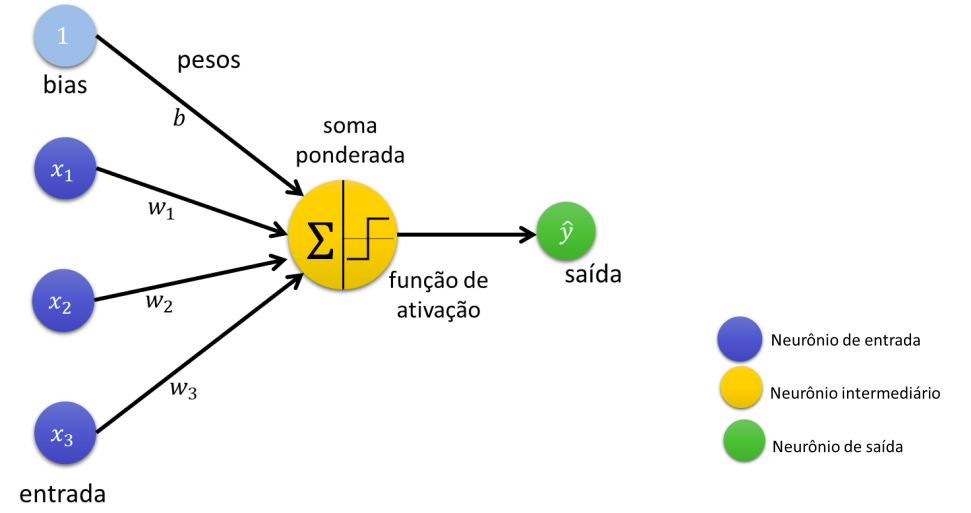
\includegraphics[width=1\textwidth]{figs/PERCEPTRON.png} % Substitua pelo caminho da sua imagem

\end{figure}
\end{frame}

\begin{frame}
\frametitle{Estrutura do Perceptron}
\begin{figure}
    \centering
    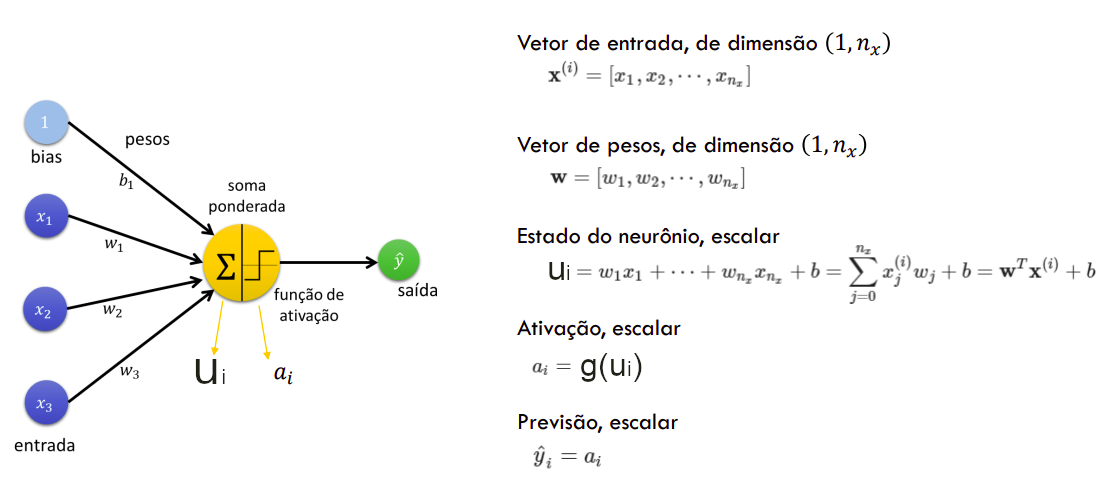
\includegraphics[width=1.1\textwidth]{figs/PERCEPTRON2.png} % Substitua pelo caminho da sua imagem

\end{figure}
\end{frame}

\begin{frame}
\frametitle{Neurônio que Implementa a Porta OR}
\begin{itemize}
    \item Considere um neurônio com duas entradas \( x_1 \) e \( x_2 \).
    \item Os pesos sinápticos são \( w_1 = 1 \) e \( w_2 = 1 \).
    \item O limiar de ativação é \( \theta = 0,5 \).
    \item A saída \( y \) é dada por:
    \[
    y = \begin{cases}
    1, & \text{se } u \geq 0, \\
    0, & \text{se } u < 0,
    \end{cases}
    \]
    onde \( u = w_1 x_1 + w_2 x_2 - \theta \).
\end{itemize}
\end{frame}

\begin{frame}
\frametitle{Cálculo da Saída para a Porta OR}
\begin{itemize}
    \item A porta OR é definida pela seguinte tabela verdade:
    \begin{table}[]
    \centering
    \begin{tabular}{cc|c}
    \( x_1 \) & \( x_2 \) & \( y \) \\
    \hline
    0 & 0 & 0 \\
    0 & 1 & 1 \\
    1 & 0 & 1 \\
    1 & 1 & 1 \\
    \end{tabular}
    \end{table}
    \item Vamos calcular a saída \( y \) para cada combinação de entradas.
\end{itemize}
\end{frame}

\begin{frame}
\frametitle{Exemplo de Cálculo}
\begin{itemize}
    \item Para \( x_1 = 0 \) e \( x_2 = 0 \):
    \[
    u = (1 \cdot 0) + (1 \cdot 0) - 0,5 = -0,5 \quad \Rightarrow \quad y = 0.
    \]
    \item Para \( x_1 = 0 \) e \( x_2 = 1 \):
    \[
    u = (1 \cdot 0) + (1 \cdot 1) - 0,5 = 0,5 \quad \Rightarrow \quad y = 1.
    \]
    \item Para \( x_1 = 1 \) e \( x_2 = 0 \):
    \[
    u = (1 \cdot 1) + (1 \cdot 0) - 0,5 = 0,5 \quad \Rightarrow \quad y = 1.
    \]
    \item Para \( x_1 = 1 \) e \( x_2 = 1 \):
    \[
    u = (1 \cdot 1) + (1 \cdot 1) - 0,5 = 1,5 \quad \Rightarrow \quad y = 1.
    \]
\end{itemize}
\end{frame}


\begin{frame}
\frametitle{Regra de Treinamento do Perceptron}
\begin{itemize}
    \item A regra de treinamento do Perceptron ajusta os pesos \( w \) e o viés \( b \) para classificar corretamente os dados de treinamento.
    \item Para um conjunto de dados linearmente separável, o algoritmo converge em um número finito de passos.
    \item A atualização dos pesos é dada por:
    \[
    w \leftarrow w + \eta (y_i - \hat{y}_i) x_i,
    \]
    onde:
    \begin{itemize}
        \item \( \eta \) é a taxa de aprendizado,
        \item \( y_i \) é a saída desejada,
        \item \( \hat{y}_i \) é a saída prevista.
    \end{itemize}
\end{itemize}
\end{frame}


\begin{frame}
\frametitle{Neurônio que Implementa a Porta AND}
\begin{itemize}
    \item Considere um neurônio com duas entradas \( x_1 \) e \( x_2 \).
    \item Inicialmente, os pesos sinápticos são \( w_1 = 0,2 \) e \( w_2 = 0,2 \).
    \item O limiar de ativação é \( \theta = 0,5 \).
    \item A saída \( y \) é dada por:
    \[
    y = \begin{cases}
    1, & \text{se } u \geq 0, \\
    0, & \text{se } u < 0,
    \end{cases}
    \]
    onde \( u = w_1 x_1 + w_2 x_2 - \theta \).
\end{itemize}
\end{frame}

\begin{frame}
\frametitle{Regra de Atualização dos Pesos}
\begin{itemize}
    \item A regra de atualização dos pesos é dada por:
    \[
    w_i \leftarrow w_i + \eta (y_{\text{esperado}} - y_{\text{calculado}}) x_i,
    \]
    onde:
    \begin{itemize}
        \item \( \eta \) é a taxa de aprendizado (vamos usar \( \eta = 0,1 \)),
        \item \( y_{\text{esperado}} \) é a saída desejada,
        \item \( y_{\text{calculado}} \) é a saída calculada pelo neurônio.
    \end{itemize}
\end{itemize}
\end{frame}

\begin{frame}
\frametitle{Passo 1: \( x_1 = 1 \), \( x_2 = 1 \)}
\begin{itemize}
    \item Saída esperada: \( y_{\text{esperado}} = 1 \).
    \item Cálculo de \( u \):
    \[
    u = (0,2 \cdot 1) + (0,2 \cdot 1) - 0,5 = -0,1 \quad \Rightarrow \quad y = 0.
    \]
    \item Erro: \( y_{\text{esperado}} - y_{\text{calculado}} = 1 - 0 = 1 \).
    \item Atualização dos pesos:
    \[
    w_1 \leftarrow 0,2 + 0,1 \cdot (1-0) \cdot 1 = 0,3,
    \]
    \[
    w_2 \leftarrow 0,2 + 0,1 \cdot (1-0) \cdot 1 = 0,3.
    \]
    \item Novos pesos: \( w_1 = 0,3 \), \( w_2 = 0,3 \).
\end{itemize}
\end{frame}

\begin{frame}
\frametitle{Passo 1.1: \( x_1 = 1 \), \( x_2 = 1 \)}
\begin{itemize}
    \item Saída esperada: \( y_{\text{esperado}} = 1 \).
    \item Cálculo de \( u \):
    \[
    u = (0,3 \cdot 1) + (0,3 \cdot 1) - 0,5 = 0,1 \quad \Rightarrow \quad y = 1.
    \]
    \item Erro: \( y_{\text{esperado}} - y_{\text{calculado}} = 1 - 1 = 0 \).
   \item Não há atualização dos pesos.
\end{itemize}
\end{frame}

\begin{frame}
\frametitle{Passo 2: \( x_1 = 1 \), \( x_2 = 0 \)}
\begin{itemize}
    \item Saída esperada: \( y_{\text{esperado}} = 0 \).
    \item Cálculo de \( u \):
    \[
    u = (0,3 \cdot 1) + (0,3 \cdot 0) - 0,5 = -0,2 \quad \Rightarrow \quad y = 0.
    \]
    \item Erro: \( y_{\text{esperado}} - y_{\text{calculado}} = 0 - 0 = 0 \).
    \item Não há atualização dos pesos.
\end{itemize}
\end{frame}

\begin{frame}
\frametitle{Passo 3: \( x_1 = 0 \), \( x_2 = 1 \)}
\begin{itemize}
    \item Saída esperada: \( y_{\text{esperado}} = 0 \).
    \item Cálculo de \( u \):
    \[
    u = (0,3 \cdot 0) + (0,3 \cdot 1) - 0,5 = -0,2 \quad \Rightarrow \quad y = 0.
    \]
    \item Erro: \( y_{\text{esperado}} - y_{\text{calculado}} = 0 - 0 = 0 \).
    \item Não há atualização dos pesos.
\end{itemize}
\end{frame}

\begin{frame}
\frametitle{Passo 4: \( x_1 = 0 \), \( x_2 = 0 \)}
\begin{itemize}
    \item Saída esperada: \( y_{\text{esperado}} = 0 \).
    \item Cálculo de \( u \):
    \[
    u = (0,3 \cdot 0) + (0,3 \cdot 0) - 0,5 = -0,5 \quad \Rightarrow \quad y = 0.
    \]
    \item Erro: \( y_{\text{esperado}} - y_{\text{calculado}} = 0 - 0 = 0 \).
    \item Não há atualização dos pesos.
\end{itemize}
\end{frame}

\begin{frame}
\frametitle{Função de Ativação}
\begin{itemize}
    \item A função de ativação \( \varphi: \mathbb{R} \to \mathbb{R} \) é aplicada à saída de um neurônio artificial.
    \item Ela introduz não linearidade no modelo, permitindo que a rede neural aprenda padrões complexos.
    \item Sem a não linearidade, uma rede neural com múltiplas camadas seria equivalente a uma única transformação linear.
\end{itemize}
\end{frame}

\begin{frame}
\frametitle{Importância da Não Linearidade}
\begin{itemize}
    \item Em redes neurais com várias camadas ocultas, a ausência de não linearidade resultaria em uma composição de transformações afins.
    \item Matematicamente, isso pode ser expresso como:
    \[
    f(x) = W_n(W_{n-1}(\dots W_1(x) + b_1) + b_{n-1}) + b_n,
    \]
    onde \( W_i \) são matrizes de pesos e \( b_i \) são vetores de viés.
    \item Sem funções de ativação não lineares, \( f(x) \) seria equivalente a uma única transformação afim:
    \[
    f(x) = W'x + b'.
    \]
\end{itemize}
\end{frame}

\begin{frame}
\frametitle{Exemplos de Funções de Ativação}
\begin{itemize}
    \item \textbf{Função Limiar (Step)}:
    \[
    \varphi(t) = \begin{cases}
    1, & t \geq 0, \\
    0, & t < 0.
    \end{cases}
    \]
    \item \textbf{Função Logística (Sigmoide)}:
    \[
    \sigma(t) = \frac{1}{1 + e^{-t}}.
    \]
    \item \textbf{Função ReLU (Rectified Linear Unit)}:
    \[
    \text{ReLU}(t) = \max(0, t).
    \]
\end{itemize}
\end{frame}

\begin{frame}
\frametitle{Impacto na Aprendizagem}
\begin{itemize}
    \item A não linearidade introduzida pela função de ativação permite que a rede neural modele relações complexas entre entradas e saídas.
    \item Sem funções de ativação não lineares, a rede não seria capaz de aprender funções não lineares, limitando sua aplicabilidade.
    \item A escolha da função de ativação afeta a eficiência do treinamento e a capacidade de generalização do modelo.
\end{itemize}
\end{frame}



\begin{frame}
\frametitle{Limitações do Perceptron}
\begin{itemize}
    \item O Perceptron só pode classificar dados linearmente separáveis.
    \item Ele não consegue resolver problemas não lineares, como o problema do XOR (ou-exclusivo).
    \item Essa limitação foi destacada por Minsky e Papert em 1969, o que levou a um declínio temporário no interesse por redes neurais.
\end{itemize}
\end{frame}
\subsection{RNA}
\begin{frame}
\frametitle{Definição Matemática de uma RNA}
\begin{itemize}
    \item Uma Rede Neural Artificial (RNA) pode ser vista como uma função \( f \) que mapeia um conjunto de dados de entrada \( X \) para um conjunto de saídas \( Y \).
    \item Formalmente, a RNA é uma função:
    \[
    f: \mathbb{R}^{n_x} \to \mathbb{R}^{n_y},
    \]
    onde:
    \begin{itemize}
        \item \( n_x \) é o número de features (entradas),
        \item \( n_y \) é o número de saídas.
    \end{itemize}
\end{itemize}
\end{frame}

\begin{frame}
\frametitle{Representação dos Dados}
\begin{itemize}
    \item Os dados de entrada são representados por uma matriz \( X \in \mathbb{R}^{n_x \times m} \), onde:
    \begin{itemize}
        \item \( n_x \) é o número de features por exemplo,
        \item \( m \) é o número total de exemplos de treinamento.
    \end{itemize}
    \item As saídas desejadas são representadas por uma matriz \( Y \in \mathbb{R}^{n_y \times m} \), onde:
    \begin{itemize}
        \item \( n_y \) é o número de saídas por exemplo.
    \end{itemize}
\end{itemize}
\end{frame}


\begin{frame}
\frametitle{Processo de Aprendizagem}
\begin{itemize}
    \item A principal característica de uma rede neural é sua capacidade de aprender e melhorar o desempenho com base em estímulos externos.
    \item A aprendizagem envolve a atualização da representação interna da rede, ajustando sua arquitetura e os pesos das conexões entre neurônios.
    \item Esse processo permite que a rede desempenhe tarefas específicas de forma mais eficiente ao longo do tempo.
\end{itemize}
\end{frame}

\begin{frame}
\frametitle{Atualização da Representação Interna}
\begin{itemize}
    \item A aprendizagem ocorre por meio da modificação da arquitetura da rede e do ajuste dos pesos sinápticos.
    \item As regras de aprendizagem determinam como os pesos são atualizados em resposta aos erros ou estímulos externos.
    \item Essas regras são essenciais para garantir que a rede se adapte e melhore seu desempenho.
\end{itemize}
\end{frame}

\begin{frame}
\frametitle{Tipos de Regras de Aprendizagem}
\begin{itemize}
    \item \textbf{Aprendizagem por Correção de Erro}:
    \begin{itemize}
        \item Utilizada em treinamento supervisionado.
        \item Os pesos são ajustados com base no erro, que é a diferença entre a saída da rede e o valor esperado.
        \item O erro é minimizado gradualmente ao longo dos ciclos de treinamento.
    \end{itemize}
    \item Outras regras de aprendizagem incluem:
    \begin{itemize}
        \item Aprendizagem Hebbiana,
        \item Aprendizagem Competitiva,
        \item Aprendizagem por Reforço.
    \end{itemize}
\end{itemize}
\end{frame}

\begin{frame}
\frametitle{Aprendizagem por Correção de Erro}
\begin{itemize}
    \item A regra de correção de erro é uma das mais comuns em redes neurais supervisionadas.
    \item O erro é calculado como:
    \[
    \text{Erro} = y_{\text{esperado}} - y_{\text{calculado}}.
    \]
    \item Os pesos são atualizados usando a fórmula:
    \[
    w_i \leftarrow w_i + \eta \cdot \text{Erro} \cdot x_i,
    \]
    onde \( \eta \) é a taxa de aprendizado e \( x_i \) é a entrada.
\end{itemize}
\end{frame}

\begin{frame}
\frametitle{Treinamento da RNA}
\begin{itemize}
    \item Para que a RNA aprenda a mapear \( X \) para \( Y \), ela precisa ser treinada.
    \item O treinamento é um processo de otimização que minimiza uma função de perda \( \mathcal{L} \), que mede a diferença entre as saídas previstas \( \hat{Y} \) e as saídas desejadas \( Y \):
    \[
    \mathcal{L}(Y, \hat{Y}) = \frac{1}{m} \sum_{i=1}^m \| y_i - \hat{y}_i \|^2.
    \]
    \item Durante o treinamento, os parâmetros da RNA (pesos e vieses) são ajustados para minimizar \( \mathcal{L} \).
\end{itemize}
\end{frame}

\begin{frame}
\frametitle{Aprendizado Supervisionado}
\begin{itemize}
    \item O treinamento de uma RNA é tipicamente supervisionado, o que requer um conjunto de dados rotulados \( \{(x_i, y_i)\}_{i=1}^m \).
    \item A cada iteração, a RNA gera uma saída \( \hat{y}_i \) para a entrada \( x_i \).
    \item A diferença entre \( y_i \) e \( \hat{y}_i \) é usada para atualizar os parâmetros da rede via retropropagação.
\end{itemize}
\end{frame}


\subsection{Multi Layer Perceptron}

\begin{frame}
\frametitle{Introdução ao Multi-Layer Perceptron (MLP)}
\begin{itemize}
    \item As limitações do Perceptron simples levaram ao desenvolvimento de redes neurais com múltiplas camadas, como o Adaline e o MLP.
    \item O MLP (Multi-Layer Perceptron) foi proposto por Rumelhart e McClelland em 1986, com base em trabalhos anteriores de Widrow e Hoff (1960).
    \item O MLP é composto por várias camadas de neurônios artificiais, permitindo a modelagem de funções não lineares complexas.
\end{itemize}
\end{frame}

\begin{frame}
\frametitle{Introdução ao MLP}
\begin{itemize}
    \item O Multi-Layer Perceptron (MLP) é uma rede neural artificial com múltiplas camadas de neurônios.
    \item Ele é composto por:
    \begin{itemize}
        \item Uma camada de entrada,
        \item Uma ou mais camadas ocultas,
        \item Uma camada de saída.
    \end{itemize}
    \item A topologia do MLP permite a modelagem de funções não lineares complexas.
\end{itemize}
\end{frame}

\begin{frame}
\frametitle{Topologia do MLP}
\begin{itemize}
    \item A topologia de um MLP é definida pela organização das camadas e pelas conexões entre os neurônios.
    \item Cada camada é composta por um conjunto de neurônios que processam informações e passam os resultados para a camada seguinte.
    \item As conexões entre os neurônios são representadas por pesos sinápticos.
\end{itemize}
\end{frame}

\begin{frame}
\frametitle{Topologia do MLP}
\begin{figure}
    \centering
    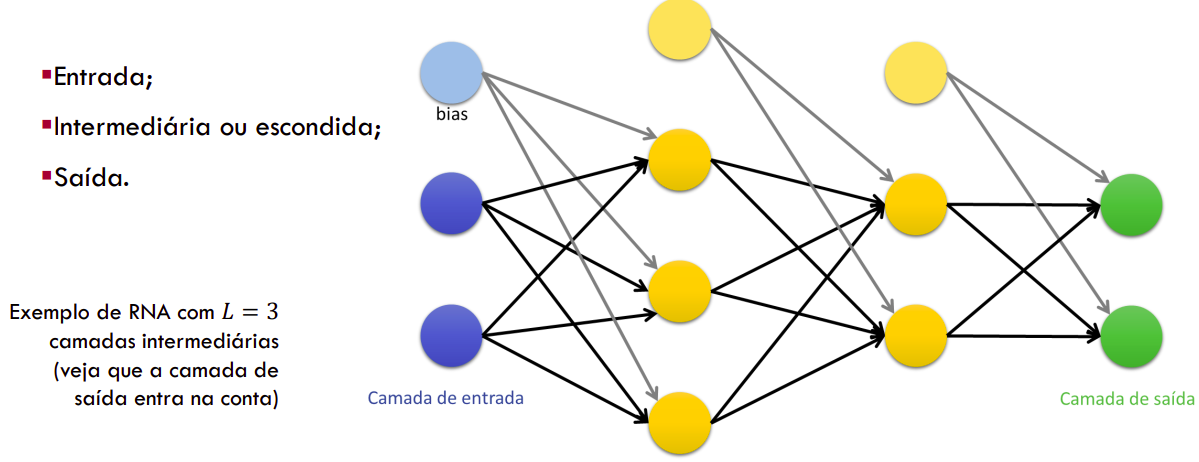
\includegraphics[width=1.05\textwidth]{figs/topologia.png}
\end{figure}
\end{frame}

\begin{frame}
\frametitle{Definição Matemática de uma Camada}
\begin{itemize}
    \item Uma camada de \( m \) neurônios pode ser representada por uma função \( L: \mathbb{R}^n \to \mathbb{R}^m \).
    \item A função de uma camada é dada por:
    \[
    L(x) = \varphi(Wx - b),
    \]
    onde:
    \begin{itemize}
        \item \( W \in \mathbb{R}^{m \times n} \) é a matriz de pesos sinápticos,
        \item \( b \in \mathbb{R}^m \) é o vetor de vieses,
        \item \( \varphi \) é a função de ativação aplicada componente a componente.
    \end{itemize}
\end{itemize}
\end{frame}

\begin{frame}
\frametitle{Camada Densa ou Totalmente Conectada}
\begin{itemize}
    \item Uma camada é chamada de \textbf{densa} ou \textbf{totalmente conectada} se a matriz \( W \) é uma matriz cheia, ou seja, todos os elementos da matriz podem ser diferentes de zero.
    \item Isso significa que cada neurônio na camada recebe entradas de todos os neurônios da camada anterior.
    \item Matematicamente, a densidade da camada é expressa pela estrutura completa da matriz \( W \).
\end{itemize}
\end{frame}

\begin{frame}
\frametitle{Exemplo de MLP com Duas Camadas}
\begin{itemize}
    \item Considere um MLP com duas camadas:
    \begin{itemize}
        \item A primeira camada \( L_1: \mathbb{R}^n \to \mathbb{R}^k \) com função de ativação \( \varphi_1 \).
        \item A segunda camada \( L_2: \mathbb{R}^k \to \mathbb{R}^m \) com função de ativação \( \varphi_2 \).
    \end{itemize}
    \item A função total do MLP é dada por:
    \[
    f(x) = L_2(L_1(x)) = \varphi_2(W_2 \varphi_1(W_1 x - b_1) - b_2).
    \]
    \item Essa composição de camadas permite a modelagem de funções não lineares complexas.
\end{itemize}
\end{frame}

\begin{frame}
\frametitle{Papel das Camadas}
\begin{itemize}
    \item As primeiras camadas (\( L_1, L_2, \ldots \)) atuam como \textbf{extratores de características}, transformando a entrada em representações intermediárias.
    \item As últimas camadas (\( L_{K-1}, L_K \)) realizam a tarefa de aprendizado de máquina, como classificação ou regressão.
    \item A camada \( L_0 \) pode ser incluída como a identidade, representando a entrada original.
\end{itemize}
\end{frame}

\begin{frame}
\frametitle{Redes Neurais Profundas}
\begin{itemize}
    \item Uma rede neural é considerada profunda (\textbf{deep}) quando possui três ou mais camadas (\( K \geq 3 \)).
    \item Redes profundas são capazes de modelar funções altamente não lineares e capturar relações complexas nos dados.
    \item A profundidade da rede permite a extração de características hierárquicas, onde camadas iniciais detectam padrões simples e camadas posteriores combinam esses padrões em representações mais complexas.
\end{itemize}
\end{frame}

\begin{frame}
\frametitle{Exemplo de Rede Profunda}
\begin{itemize}
    \item Considere uma rede com \( K = 4 \) camadas:
    \begin{itemize}
        \item \( L_1: \mathbb{R}^n \to \mathbb{R}^{h_1} \),
        \item \( L_2: \mathbb{R}^{h_1} \to \mathbb{R}^{h_2} \),
        \item \( L_3: \mathbb{R}^{h_2} \to \mathbb{R}^{h_3} \),
        \item \( L_4: \mathbb{R}^{h_3} \to \mathbb{R}^m \).
    \end{itemize}
    \item A função total da rede é:
    \[
    N(x) = L_4(L_3(L_2(L_1(x)))).
    \]
    \item Cada camada aplica uma transformação não linear, permitindo que a rede aprenda representações complexas.
\end{itemize}
\end{frame}

\begin{frame}
\frametitle{Treinamento de Redes Neurais}
\begin{itemize}
    \item O treinamento de uma rede neural (superficial ou profunda) envolve a minimização de uma função de perda.
    \item Em problemas de regressão, a função de perda comum é o \textbf{Erro Quadrático Médio (MSE)}:
    \[
    \text{MSE} = \frac{1}{m} \sum_{i=1}^m (y_i - \hat{y}_i)^2,
    \]
    onde \( y_i \) é o valor esperado e \( \hat{y}_i \) é a saída da rede.
    \item Em problemas de classificação, a função de perda comum é a \textbf{Entropia Cruzada}:
    \[
    \text{Entropia Cruzada} = -\sum_{i=1}^m y_i \log(\hat{y}_i).
    \]
\end{itemize}
\end{frame}

\begin{frame}
\frametitle{Formulação do Problema de Otimização}
\begin{itemize}
    \item O treinamento é formulado como um problema de otimização irrestrito nos parâmetros da rede (pesos \( W \) e vieses \( b \)).
    \item O objetivo é encontrar os parâmetros que minimizam a função de perda:
    \[
    \min_{W, b} \mathcal{L}(W, b),
    \]
    onde \( \mathcal{L} \) é a função de perda.
    \item Devido ao grande número de parâmetros, métodos baseados no gradiente são utilizados.
\end{itemize}
\end{frame}

\begin{frame}
\frametitle{Métodos Baseados no Gradiente}
\begin{itemize}
    \item O gradiente da função de perda em relação aos parâmetros é calculado usando a \textbf{regra da cadeia}.
    \item O gradiente é dado por:
    \[
    \nabla_{W, b} \mathcal{L} = \left( \frac{\partial \mathcal{L}}{\partial W}, \frac{\partial \mathcal{L}}{\partial b} \right).
    \]
    \item O cálculo do gradiente é realizado de forma eficiente usando o algoritmo de retropropagação (\textit{backpropagation}).
\end{itemize}
\end{frame}

\begin{frame}
\frametitle{Algoritmo de Retropropagação}
\begin{itemize}
    \item O algoritmo de retropropagação consiste em duas fases:
    \begin{itemize}
        \item \textbf{Fase Forward}: Calcula a saída da rede para uma dada entrada.
        \item \textbf{Fase Backward}: Propaga o erro da saída para as camadas anteriores, calculando os gradientes.
    \end{itemize}
    \item O gradiente é usado para atualizar os pesos e vieses:
    \[
    W \leftarrow W - \eta \frac{\partial \mathcal{L}}{\partial W}, \quad b \leftarrow b - \eta \frac{\partial \mathcal{L}}{\partial b},
    \]
    onde \( \eta \) é a taxa de aprendizado.
\end{itemize}
\end{frame}

\begin{frame}
\frametitle{Ilustração do Algoritmo de Retropropagação}
Veja o GIF animado:

\end{frame}
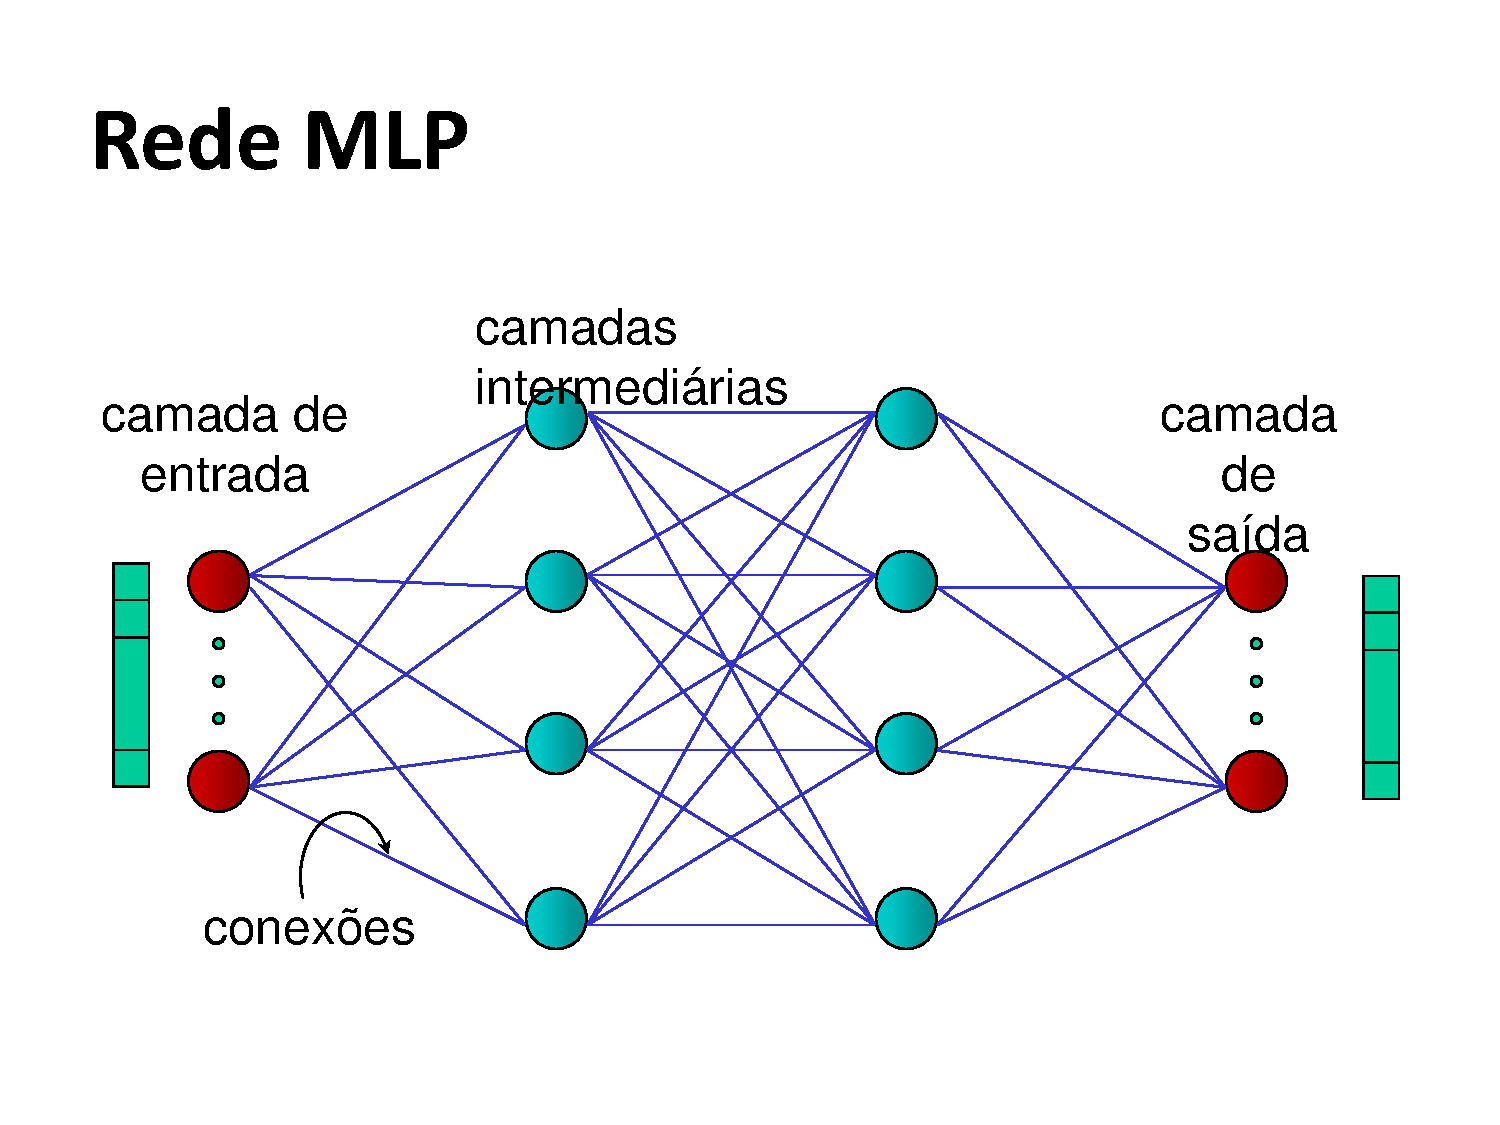
\includepdf[pages=-, frame]{figs/retropropagacao.pdf}

\begin{frame}
\frametitle{Ilustração do Algoritmo de Retropropagação}
\begin{itemize}
    \item A figura abaixo ilustra o fluxo de informações no algoritmo de retropropagação:
    \begin{figure}
        \centering
        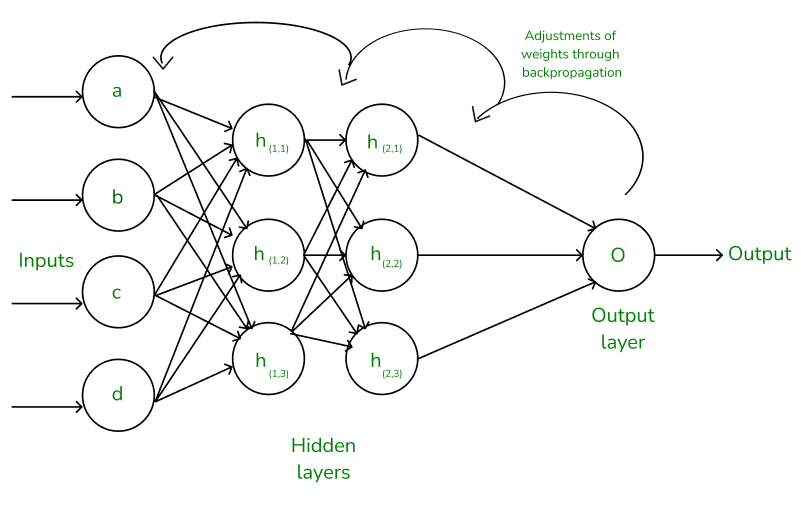
\includegraphics[width=0.9\textwidth]{figs/backpropagation.png} % Substitua pelo caminho da imagem

    \end{figure}
    \item A imagem mostra como o erro é propagado da camada de saída para as camadas anteriores, permitindo o cálculo dos gradientes.
\end{itemize}
\end{frame}

\begin{frame}
\frametitle{Conclusão}
\begin{itemize}
    \item O treinamento de redes neurais é um problema de otimização que busca minimizar uma função de perda.
    \item Métodos baseados no gradiente, como o algoritmo de retropropagação, são essenciais para o treinamento eficiente de redes neurais.
    \item A escolha da função de perda e da taxa de aprendizado é crucial para o desempenho da rede.
\end{itemize}
\end{frame}

\begin{frame}
\frametitle{RNA na prática}
\begin{itemize}
    \item sklearn
    \item keras
\end{itemize}
\end{frame}

\section{Unsupervised learning}
\subsection{Conceitos Fundamentais}
\begin{frame}
\centering
\Huge
\textbf{Unsupervised\\ Learning}
\end{frame}

\begin{frame}
\frametitle{O Que é Aprendizado Não Supervisionado?}
\begin{itemize}
    \item O aprendizado não supervisionado é um tipo de aprendizado de máquina onde o modelo é treinado com dados \textbf{não rotulados}.
    \item O objetivo é encontrar padrões, estruturas ou relações nos dados sem a necessidade de rótulos pré-definidos.
    \item É amplamente utilizado em tarefas como:
    \begin{itemize}
        \item Agrupamento (clustering),
        \item Redução de dimensionalidade,
        \item Detecção de anomalias.
    \end{itemize}
\end{itemize}
\end{frame}

\begin{frame}
\frametitle{Formulação Matemática}
\begin{itemize}
    \item Dado um conjunto de dados \( X = \{x_1, x_2, \dots, x_n\} \), onde \( x_i \in \mathbb{R}^d \), o objetivo é aprender uma representação ou estrutura subjacente.
    \item Em problemas de agrupamento, por exemplo, busca-se particionar \( X \) em \( k \) grupos \( C_1, C_2, \dots, C_k \), onde:
    \[
    \bigcup_{i=1}^k C_i = X \quad \text{e} \quad C_i \cap C_j = \emptyset \quad \text{para} \quad i \neq j.
    \]
    \item A qualidade do agrupamento é medida por uma função de custo, como a soma dos quadrados intra-cluster:
    \[
    \mathcal{J} = \sum_{i=1}^k \sum_{x \in C_i} \|x - \mu_i\|^2,
    \]
    onde \( \mu_i \) é o centróide do cluster \( C_i \).
\end{itemize}
\end{frame}
\subsection{K-Means}
\begin{frame}
\frametitle{Exemplo: Algoritmo K-Means}
\begin{itemize}
    \item O K-Means é um algoritmo clássico de agrupamento não supervisionado.
    \item Dado um número \( k \) de clusters, o algoritmo minimiza a função de custo:
    \[
    \mathcal{J} = \sum_{i=1}^k \sum_{x \in C_i} \|x - \mu_i\|^2.
    \]
    \item Os passos do algoritmo são:
    \begin{enumerate}
        \item Inicializar os centróides \( \mu_1, \mu_2, \dots, \mu_k \).
        \item Atribuir cada ponto \( x \) ao cluster mais próximo.
        \item Atualizar os centróides como a média dos pontos no cluster.
        \item Repetir até convergência.
    \end{enumerate}
\end{itemize}
\end{frame}

\begin{frame}
\frametitle{Ilustração do K-Means}
\begin{itemize}
    \item A figura abaixo ilustra o funcionamento do algoritmo K-Means:
    \begin{figure}
        \centering
        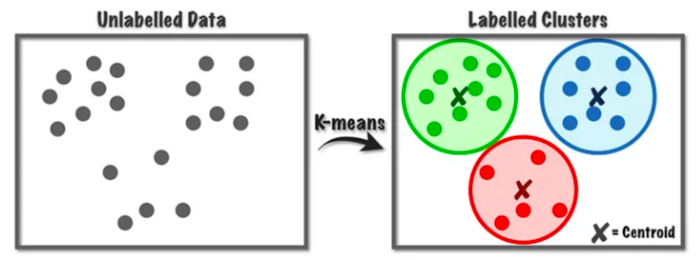
\includegraphics[width=0.7\textwidth]{figs/kmeans.png} % Substitua pelo caminho da imagem
        \caption{Passos do algoritmo K-Means: (1) Inicialização dos centróides, (2) Atribuição de pontos aos clusters, (3) Atualização dos centróides.}
        \label{fig:kmeans}
    \end{figure}
    \item O algoritmo alterna entre atribuir pontos aos clusters e atualizar os centróides até convergir.
\end{itemize}
\end{frame}

\subsection{PCA}

\begin{frame}
\frametitle{Redução de Dimensionalidade}
\begin{itemize}
    \item Outra tarefa comum no aprendizado não supervisionado é a redução de dimensionalidade.
    \item O objetivo é mapear os dados de um espaço de alta dimensão \( \mathbb{R}^d \) para um espaço de menor dimensão \( \mathbb{R}^k \), onde \( k < d \).
    \item Um método popular é a \textbf{Análise de Componentes Principais} (PCA), que busca encontrar as direções de máxima variância nos dados.
    \item Matematicamente, o PCA resolve o problema de autovalores:
    \[
    \Sigma v = \lambda v,
    \]
    onde \( \Sigma \) é a matriz de covariância dos dados e \( v \) são os autovetores.
\end{itemize}
\end{frame}

\begin{frame}
\frametitle{Ilustração do PCA}
\begin{itemize}
    \item A figura abaixo ilustra a projeção dos dados em componentes principais:
    \begin{figure}
        \centering
        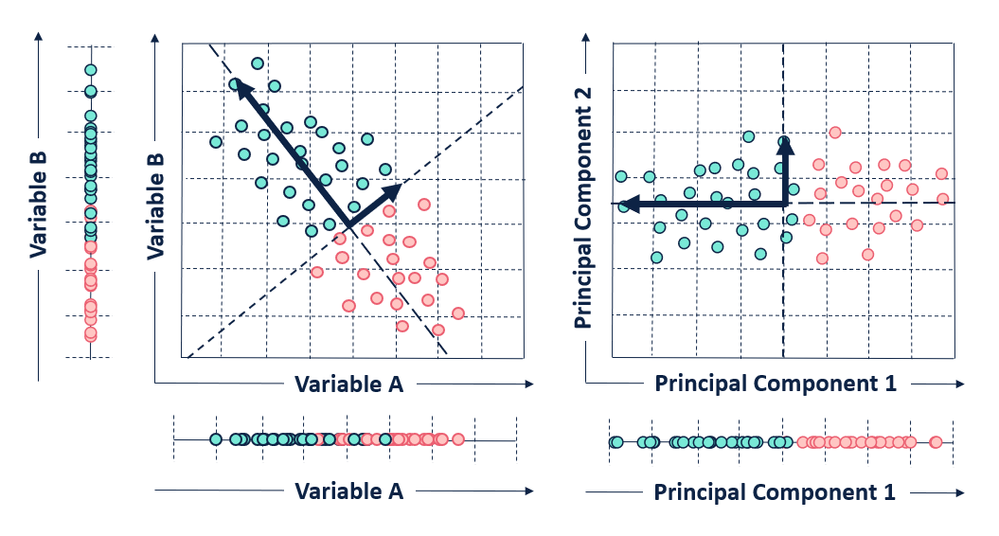
\includegraphics[width=0.7\textwidth]{figs/pca.png} % Substitua pelo caminho da imagem
        \caption{os dados são projetados em duas componentes principais.}
        \label{fig:pca}
    \end{figure}
    \item As componentes principais são as direções que maximizam a variância dos dados.
\end{itemize}
\end{frame}

\begin{frame}
\frametitle{Ilustração do PCA}
    \begin{figure}
        \centering
        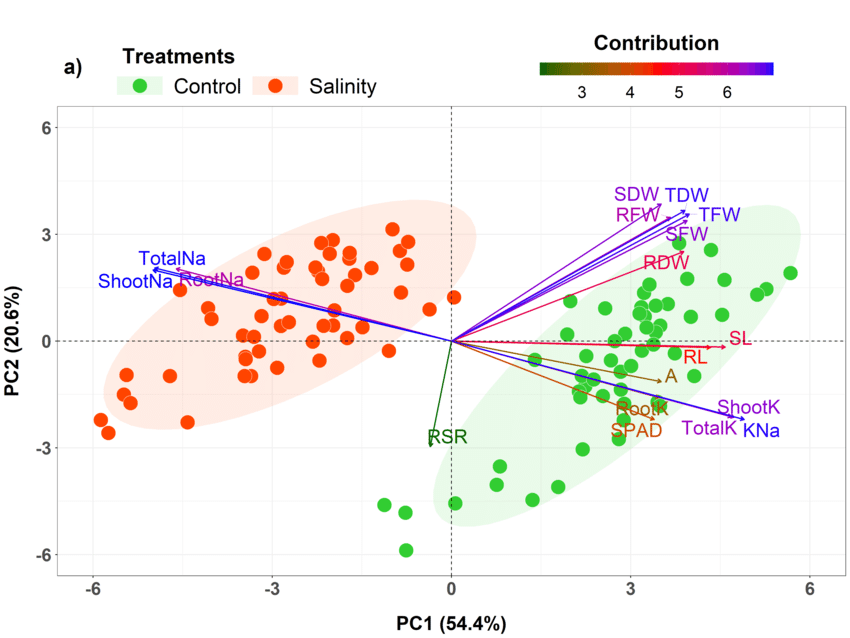
\includegraphics[width=0.7\textwidth]{figs/pca2.png}
    \end{figure}

\end{frame}

\begin{frame}
\frametitle{Conclusão}
\begin{itemize}
    \item O aprendizado não supervisionado é essencial para explorar dados não rotulados e descobrir padrões ocultos.
    \item Técnicas como agrupamento e redução de dimensionalidade são fundamentais em muitas aplicações.
    \item A formulação matemática desses métodos permite a otimização e a interpretação dos resultados.
\end{itemize}
\end{frame}



\section{Referências Bibliográficas}
\begin{frame}[t,allowframebreaks]
\frametitle{Referências}
%\bibliographystyle{amsalpha}
%\bibliography{bibfile}
\begin{thebibliography}{*}

         \bibitem[A01]{A01} Chollet, F. (2021). Deep Learning with Python, Second Edition. Shelter Island, NY: Manning Publications.
        \bibitem[A02]{A02} Géron, A. (2019). Hands-On Machine Learning with Scikit-Learn, Keras, and TensorFlow. Sebastopol, CA: O'Reilly Media..
        \bibitem[A03]{A03} Russell, S., \& Norvig, P. (2021). Artificial Intelligence: A Modern Approach (4ª ed.). Hoboken, NJ: Pearson.
        \bibitem[A04]{A04}Moroney, L. (2020). AI and Machine Learning for Coders. Sebastopol, CA: O'Reilly Media.




\end{thebibliography}
\end{frame}
\section{}

%remover logo
\setbeamertemplate{logo}{}

\begin{frame}
\titlepage
\end{frame}

\end{document}
